%%%%%%%%%%%%%%%%%%%%%%%%%%%%%%%%%%%%%%%%%
% Short Sectioned Assignment LaTeX Template Version 1.0 (5/5/12)
% This template has been downloaded from: http://www.LaTeXTemplates.com
% Original author:  Frits Wenneker (http://www.howtotex.com)
% License: CC BY-NC-SA 3.0 (http://creativecommons.org/licenses/by-nc-sa/3.0/)
%%%%%%%%%%%%%%%%%%%%%%%%%%%%%%%%%%%%%%%%%

%----------------------------------------------------------------------------------------
%	PACKAGES AND OTHER DOCUMENT CONFIGURATIONS
%----------------------------------------------------------------------------------------

\documentclass[paper=a4, fontsize=10pt]{article} % A4 paper and 11pt font size

% ---- Entrada y salida de texto -----

\usepackage[T1]{fontenc} % Use 8-bit encoding that has 256 glyphs
\usepackage[utf8]{inputenc}
%\usepackage{fourier} % Use the Adobe Utopia font for the document - comment this line to return to the LaTeX default

% ---- Idioma --------

\usepackage[spanish, es-tabla]{babel} % Selecciona el español para palabras introducidas automáticamente, p.ej. "septiembre" en la fecha y especifica que se use la palabra Tabla en vez de Cuadro

% ---- Otros paquetes ----

\usepackage{amsmath,amsfonts,amsthm} % Math packages
%\usepackage{graphics,graphicx, floatrow} %para incluir imágenes y notas en las imágenes
\usepackage{graphics,graphicx, float, url} %para incluir imágenes y colocarlas

% Para hacer tablas comlejas
%\usepackage{multirow}
%\usepackage{threeparttable}

%\usepackage{sectsty} % Allows customizing section commands
%\allsectionsfont{\centering \normalfont\scshape} % Make all sections centered, the default font and small caps

\usepackage{fancyhdr} % Custom headers and footers
\pagestyle{fancyplain} % Makes all pages in the document conform to the custom headers and footers
\fancyhead{} % No page header - if you want one, create it in the same way as the footers below
\fancyfoot[L]{} % Empty left footer
\fancyfoot[C]{} % Empty center footer
\fancyfoot[R]{\thepage} % Page numbering for right footer
\renewcommand{\headrulewidth}{0pt} % Remove header underlines
\renewcommand{\footrulewidth}{0pt} % Remove footer underlines
\setlength{\headheight}{13.6pt} % Customize the height of the header

\numberwithin{equation}{section} % Number equations within sections (i.e. 1.1, 1.2, 2.1, 2.2 instead of 1, 2, 3, 4)
\numberwithin{figure}{section} % Number figures within sections (i.e. 1.1, 1.2, 2.1, 2.2 instead of 1, 2, 3, 4)
\numberwithin{table}{section} % Number tables within sections (i.e. 1.1, 1.2, 2.1, 2.2 instead of 1, 2, 3, 4)

\setlength\parindent{0pt} % Removes all indentation from paragraphs - comment this line for an assignment with lots of text

\newcommand{\horrule}[1]{\rule{\linewidth}{#1}} % Create horizontal rule command with 1 argument of height

\usepackage{url} %bibliografía
\usepackage{appendix}
\usepackage{sectsty}
\usepackage{listings}
\usepackage{xcolor}
\usepackage{colortbl}
\usepackage{breakurl}
%\usepackage{hyperref}
%\usepackage[breaklinks=true]{hyperref}
\usepackage[hidelinks]{hyperref} 
\usepackage{fancyvrb}
\usepackage{color}

\usepackage{multirow} % para las tablas


\usepackage{anysize}
\marginsize{3cm}{3cm}{2.5cm}{2.5cm} %izq, derecha, arriba
% Se limpia la cabecera y el pie de página para poder rehacerlos luego.

% Espacios en el documento:
\linespread{1}                        % Espacio entre líneas.
\setlength\parindent{0pt}               % Selecciona la indentación para cada inicio de párrafo.


\lstset{
        tabsize=2, % tab = 2 espacios
        backgroundcolor=\color[HTML]{F0F0F0}, % color de fondo
        captionpos=b, % posición de pie de código, b=debajo
        basicstyle=\ttfamily, % estilo de letra general
        columns=fixed, % columnas alineadas
        extendedchars=true, % ASCII extendido
        breaklines=true, % partir líneas
        %prebreak = \raisebox{0ex}[0ex][0ex]{\ensuremath{\hookleftarrow}}, % marcar final de línea con flecha
        showtabs=false, % no marcar tabulación
        showspaces=false, % no marcar espacios
        keywordstyle=\bfseries\color[HTML]{007020}, % estilo de palabras clave
        commentstyle=\itshape\color[HTML]{60A0B0}, % estilo de comentarios
        stringstyle=\color[HTML]{4070A0}, % estilo de strings
}

\renewcommand{\appendixname}{Anexos}
\renewcommand{\appendixtocname}{Anexos}
\renewcommand{\appendixpagename}{Anexos}

\title{	
\normalfont \normalsize 
\textsc{{\bf Sistemas multimedia (2018-2019)} \\ Grado en Ingeniería Informática \\ Universidad de Granada} \\ [25pt] % Your university, school and/or dbrewepartment name(s)
\horrule{0.5pt} \\[0.4cm] % Thin top horizontal rule
\huge Domentación Paint. Práctica de Evaluación. \\ % The assignment title
\horrule{2pt} \\[0.5cm] % Thick bottom horizontal rule
}
\author{Montserrat Rodríguez Zamorano} % Nombre y apellidos
\date{\normalsize\today} % Incluye la fecha actual

\begin{document}
\pagestyle{empty}
\maketitle
\vskip1cm
\clearpage
\tableofcontents
\clearpage
%\vskip0.3cm
%\begin{figure}[H]
 % \centering
  %  \includegraphics[width=0.8\textwidth]{}
 % \caption{Diseño conceptual}
 % \label{diseño}
%\end{figure}
\setcounter{page}{1}
\pagestyle{plain}
\section{Descripción del sistema}
Para la evaluación de la asignatura de \textit{Sistemas multimedia} se quiere realizar una aplicación multimedia que permita gestionar gráficos, imágenes, sonido y vídeo. Se podrá crear, editar, procesar y visualizar contenido multimedia de distintos tipos.
\vskip0.3cm
Esta aplicación tendrá una ventana principal con diferentes barras de herramientas y botones que permitirán realizar las distintas operaciones sobre el contenido multimedia. Se intentará que la interfaz sea lo más intuitiva posible y facilitar así el uso de la aplicación al usuario final.
\vskip0.3cm
Con este fin, se realiza una aplicación que se llamará \textit{Paint}.
\section{Requisitos}
\subsection{Requisitos funcionales}
\subsubsection{Carácter general}
\begin{itemize}
\item{\textbf{[RFCG-1]} Creación de una nueva imagen en una nueva ventana.}
\item{\textbf{[RFCG-2} Abrir un fichero de imagen.}
\item{\textbf{[RFCG-3]} Abrir un fichero de sonido.}
\item{\textbf{[RFCG-4]} Abrir un fichero de vídeo.}
\item{\textbf{[RFCG-5]} Guardar una imagen y sus figuras dibujadas.}
\item{\textbf{[RFCG-6]} Ocultar las barras de herramientas.}
\item{\textbf{[RFCG-7]} Visualizar las barras de herramientas.}
\item{\textbf{[RFCG-8]} Consultar el nombre del programa, versión y autor.}
\end{itemize}
\subsubsection{Dibujo}
\begin{itemize}
\item{\textbf{[RFD-1]} Dibujar las siguientes formas geométricas con sus propios atributos independientes.
\begin{itemize}
\item{Línea.}
\item{Rectángulo.}
\item{Elipse.}
\item{Rectángulo con esquinas redondeadas.}
\end{itemize}
}
\item{\textbf{[RFD-2]} El lienzo mantendrá todas las figuras que se vayan dibujando.}
\item{\textbf{[RFD-3]} Elegir el color de trazo de dibujo.
\begin{itemize}
\item{Rojo.}
\item{Azul.}
\item{Negro.}
\item{Blanco.}
\item{Verde.}
\end{itemize}
}
\item{\textbf{[RFD-4]} No rellenar la figura.}
\item{\textbf{[RFD-5]} Rellenar con color la figura.
\begin{itemize}
\item{Rojo.}
\item{Azul.}
\item{Negro.}
\item{Blanco.}
\item{Verde.}
\end{itemize}
}
\item{\textbf{[RFD-6]} Colorear con diferentes tipos de relleno la figura.}
\begin{itemize}
\item{Degradado horizontal.}
\item{Degradado vertical.}
\item{Degradado diagonal.}
\end{itemize}
\item{\textbf{[RFD-7]} Escoger el tipo de línea con la que se pintará la figura.}
\begin{itemize}
\item{Continua.}
\item{Discontinua.}
\item{Punteada.}
\end{itemize}
\item{\textbf{[RFD-8]} Seleccionar una figura dibujada.}
\item{\textbf{[RFD-9]} Editar una figura dibujada.}
\item{\textbf{[RFD-10]} Mover una figura dibujada.}
\item{\textbf{[RFD-11]} Consultar la lista de figuras dibujadas.}
\item{\textbf{[RFD-12]} Consultar los atributos de una figura dibujada.}
\item{\textbf{[RFD-13]} Asociar un grado de transparencia a una figura.}
\item{\textbf{[RFD-14]} Activar alisado de bordes de una figura.}
\item{\textbf{[RFD-15]} Desactivar alisado de bordes de una figura.}
\item{\textbf{[RFD-16]} Consultar los atributos de dibujo activo en un lienzo.}
\end{itemize}
\subsubsection{Procesamiento de imágenes}
\begin{itemize}
\item{\textbf{[RFPI-1]} Duplicar una imagen.}
\item{\textbf{[RFPI-2]} Modificar el brillo de una imagen.}
\item{\textbf{[RFPI-3]} Aplicar filtro para emborronar una imagen.}
\item{\textbf{[RFPI-4]} Aplicar filtro para enfocar una imagen.}
\item{\textbf{[RFPI-5]} Aplicar filtro de relieve a una imagen.}
\item{\textbf{[RFPI-6]} Aplicar contraste a una imagen.}
\item{\textbf{[RFPI-7]} Iluminar una imagen.}
\item{\textbf{[RFPI-8]} Oscurecer una imagen.}
\item{\textbf{[RFPI-9]} Extraer las bandas de una imagen.}
\item{\textbf{[RFPI-10]} Invertir los colores de una imagen.}
\item{\textbf{[RFPI-11]} Convertir una imagen a los siguientes espacios:
\begin{itemize}
\item{RGB}
\item{YCC}
\item{GRAY}
\end{itemize}
}
\item{\textbf{[RFPI-12]} Girar una imagen a cualquier ángulo.}
\item{\textbf{[RFPI-13]} Tintar una imagen.}
\item{\textbf{[RFPI-14]} Escoger nivel y color de tintado de una imagen.}
\item{\textbf{[RFPI-15]} Ecualizar una imagen.}
\item{\textbf{[RFPI-16]} Umbralizar una imagen en niveles de gris.}
\item{\textbf{[RFPI-17]} Escoger nivel de umbralización.}
\item{\textbf{[RFPI-18]} Aplicar filtro sepia a una imagen.}
\item{\textbf{[RFPI-19]} Aplicar filtro violeta a una imagen.}
\item{\textbf{[RFPI-20]} Aplicar filtro potenciador del color rojo (diseño propio).}
\item{\textbf{[RFD-21]} Aplicar filtro media de bandas azul y verde (diseño propio).}
\item{\textbf{[RFPI-22]} Aplicar filtro cosinosuidal.}
\item{\textbf{[RFPI-23]} El procesamiento de imágenes no se aplicarán sobre las figuras dibujadas.}
\item{\textbf{[RFPI-24]} Escalar una imagen.}
\end{itemize}
\subsubsection{Sonido}
\begin{itemize}
\item{\textbf{[RFS-1]} Reproducir audios.}
\item{\textbf{[RFS-2]} Grabar sonidos.}
\item{\textbf{[RFS-3]} Parar la grabación.}
\item{\textbf{[RFS-4]} Parar la reproducción.}
\end{itemize}
\subsubsection{Vídeo}
\begin{itemize}
\item{\textbf{[RFV-1]} Mostrar la secuencia que capte la Webcam.}
\item{\textbf{[RFV-2]} Capturar una imagen desde la Webcam.}
\item{\textbf{[RFV-3]} Comenzar la reproducción de un vídeo.}
\item{\textbf{[RFV-4]} Parar la reproducción de un vídeo.}
\item{\textbf{[RFV-5]} Pausar la reproducción de un vídeo.}
\end{itemize}
\subsection{Requisitos no funcionales}
\begin{itemize}
\item{\textbf{[RNF-1]} Se mostrará en la barra de estado el pixel en el que está situado el ratón.}
\item{\textbf{[RNF-2]} Se habilitarán en cada momento sólo los botones que pueden utilizarse.}
\item{\textbf{[RNF-3]} Los botones tendrán asociados un \textit{ToolTipText} para facilitar el uso del programa.}
\item{\textbf{[RNF-4]} Al seleccionar una figura se activarán sus propiedades en la barra de atributos.}
\item{\textbf{[RNF-5]} Si hay una figura seleccionada, al pulsar el ratón sobre en otro punto, deberá deseleccionarse la figura.}
\item{\textbf{[RNF-6]} El título de una nueva ventana abierta será el nombre del fichero si se trata de una imagen abierta o guardada.}
\item{\textbf{[RNF-7]} El título de una nueva ventana abierta será \textit{Nueva} si se trata de una imagen creada por el usuario.}
\item{\textbf{[RNF-8]} El título de una nueva ventana abierta será \textit{Captura} si se trata de una captura captada de un vídeo o de la WebCam.}
\item{\textbf{[RNF-9]} La \textit{BoundingBox} será un rectángulo de color azul con cierto grado de transparencia, con línea discontinua.}
\item{\textbf{[RNF-10]} Cuando se cree una imagen se lanzará un diálogo que permita elegir las dimensiones de la imagen.}
\item{\textbf{[RNF-11]} Se indicará entre corchetes en el título de la ventana el espacio de color en el que está la imagen.}
\item{\textbf{[RNF-12]} Cuando se extraigan las bandas de una imagen se indicará en el título de la ventana la banda en la que se encuentra.}
\end{itemize}

\clearpage

\section{Análisis}
Se hará un análisis del problema y de las posibles soluciones, intentando que sea lo más independiente posible del lenguaje de programación. En el apartado de \textit{Diseño} se especificarán detalles relacionados con la programación.
\vskip0.3cm
En primer lugar, se plantea cómo debería ser el área de dibujo, que almacenará los atributos con los que se pintará la siguiente figura. Con este fin se desarrollará una clase \textit{Lienzo}. Esta clase será la encargada de pintar las figuras. Cada figura dibujada en el área de dibujo tendrá los atributos activos en ese momento en el lienzo, si bien sus atributos podrán modificarse a posteriori cuando se seleccione esta figura(\textbf{[RFD-8:10]}), así como consultar los atributos de cada una de las figuras dibujadas en ese lienzo (\textbf{[RFD-11,12]}).
\vskip0.3cm
La solución planteada durante el desarrollo de las prácticas no es muy flexible: la biblioteca \texttt{java.awt.Graphics} ofrece importantes limitaciones, ya que no permite que los objetos tengan propiedades de color, forma o grosor, entre otras. De esta forma, todas las figuras de un mismo lienzo se pintarán con los mismos atributos (\textbf{[RFD-1:7,13:15]}).
\vskip0.3cm
Para que cada figura tenga sus propios atributos se desarrollará una clase propia \textit{Figura}, que almacenará cada uno de los atributos de la figura y permitirá que cada figura tenga los suyos propios: color, grosor, etc. Sin embargo, la línea, por ejemplo, no puede tener relleno, por lo que no tiene sentido guardar este atributo. Se desarrollará una clase propia para cada una de las figuras que pueden dibujarse: Línea, rectángulo, elipse, rectángulo redondeado.
\vskip0.3cm
Para intentar mejorar el diseño de esta clase, en lugar de que las formas hereden directamente de \textit{Figura}, se dividirán en dos grupos: figuras rellenables y figuras lineales. De esta forma, las operaciones comunes relativas al relleno podrán realizarse en el ámbito de la figura rellenable, y no tener que implementarlas en cada una de las clases derivadas. Con esta jerarquía de clases, evitamos que figuras lineales tengan atributos que no deben tener, como por ejemplo, tipo de relleno, así como evitamos que en figuras con propiedades similares (elipse y rectángulo, por ejemplo) se repitan funciones o atributos.
\vskip0.3cm
\begin{figure}[H]
 \centering
  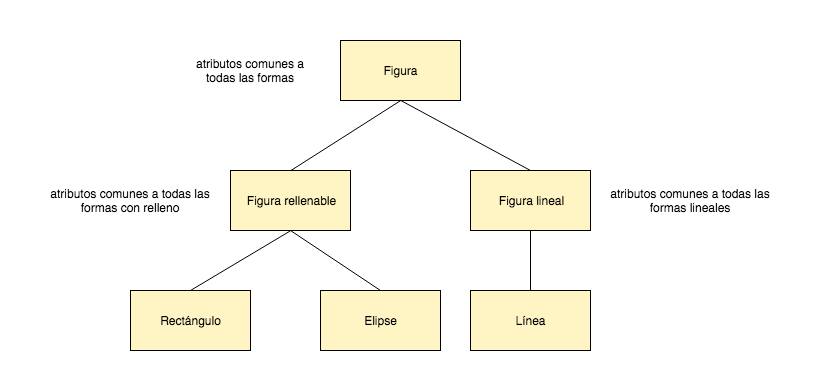
\includegraphics[width=0.8\textwidth]{esquemaFormas.png}
 \caption{Esquema del diseño de la clase \textit{Figura}}
 \label{diseño}
 \end{figure}
\vskip0.3cm
Para el procesamiento de imágenes se hará uso de las bibliotecas proporcionadas por el profesor, así como de las disponibles en \textit{Java}. Esto permitirá cubrir los requisitos (\textbf{[RFPI-1:18,22,23]}). Los requisitos (\textbf{[RFPI-19:21]}) necesitará el desarrollo de clases propias. Se darán más detalles en el apartado de diseño.
\vskip0.3cm
En cuanto al manejo de eventos, se usará en muchas ocasiones las funciones que ofrece Java para la gestión de eventos (por ejemplo, para el uso de botones en la ventana principal). Sin embargo, para la comunicación entre el lienzo y la ventana principal será necesario crear una clase manejadora para la gestión de eventos relacionados con el lienzo. La existencia de esta clase permitirá por ejemplo informar de la falta de atributos necesarios para el dibujo de las figuras y poder lanzar mensajes de error desde la ventana principal (por ejemplo: no se ha seleccionado una forma de dibujo) o informar a la ventana principal de la creación de una nueva figura, para que aparezca en una lista desplegable de figuras seleccionables. 
\vskip0.3cm
Para terminar, los requisitos de sonido y vídeo están cubiertos por las bibliotecas proporcionadas por el profesor, por lo que no se necesitará desarrollar ninguna clase adicional (\textbf{[RFV-1:5,RFS-1:4]}).
%%%%%%%%%%%%%%%%%%% DISEÑO %%%%%%%%%%%%%%%%
\clearpage
\section{Diseño}
Siguiendo la propuesta que se ha planteado en el análisis, se plantean las siguientes jerarquías de clases. Mientras la propuesta anterior intentaba ser independiente del lenguaje de programación, en este apartado se especifican aspectos concretos de la implementación en \textit{Java}.
\vskip0.3cm
Se intentará dar una descripción general, pero para más detalles es preferible consultar los diagramas de clase. Muchas de las explicaciones se han obtenido de los guiones de prácticas y apuntes de la asignatura.
\subsection{VentanaPrincipal}
La clase \texttt{VentanaPrincipal} implementará la visión principal del programa. Heredará de \texttt{JFrame} y contendrá múltiples elementos \texttt{Swing}:
\begin{itemize}
\item{\textbf{Barras de herramientas:} serán del tipo \texttt{JToolBar}, y se tratan de las barras superior, izquierda y derecha \textbf{[RFCG-6:7]}. Serán las que contendrán la mayoría de los demás elementos \texttt{Swing}.}
\item{\textbf{Barra de estado:} se trata de un elemento \texttt{JPanel} que contendrá elementos del tipo \texttt{JLabel} \textbf{[RNF-1]}. El texto de estas etiquetas indicarán, por ejemplo, que una figura ha sido añadida.}
\item{\textbf{Listas desplegables:} se utilizarán \texttt{JComboBox} para la selección de colores, tipo de relleno, tipo de línea y figuras.}
\item{\textbf{Botones \texttt{JToggleButton}:} pueden quedarse seleccionados, por lo que se utilizarán para las formas agrupándose en un \texttt{ButtonGroup}.}
\item{\textbf{Botones \texttt{JButton}:} En el caso de por ejemplo, los filtros, no tiene demasiado interés que un botón quede seleccionado, por lo que para la mayoría de las operaciones de procesamiento de imágenes se utilizará este tipo de botones \textbf{[RFCG-1:5]}.}
\item{\textbf{Escritorio:} se trata de un elemento del tipo \texttt{JDesktopPane}. Este escritorio será aquel que contendrá las ventanas multimedia de distintos tipos.}
\end{itemize}
\subsection{Lienzo}
La clase \texttt{Lienzo} heredará de \texttt{JPanel}. Esta clase tendrá asociados los atributos con los que se pintará la siguiente figura \textbf{[RFD-3:7,13:15]}, así como un vector de las figuras dibujadas \textbf{[RFD-2]}. El objeto de tipo \texttt{Lienzo} será también el que se encargue de pintar las figuras a través del método \texttt{paint}, así como de guardar la figura seleccionada y de pintar la bounding box.  
\vskip0.3cm
Es necesario distinguir entre lienzo e imagen, aunque muchas veces se utilice la palabra lienzo con el mismo significado. Se creará la clase \texttt{LienzoImagen}, que heredará de \texttt{Lienzo}. Esta clase permitirá definir un área de dibujo, la imagen, que podrá ser creada (un rectángulo blanco de unas dimensiones determinadas, simulando un lienzo real) o abierta. En el método \texttt{paint} se llamará a \texttt{clip}, de forma que no se mostrará aquello que se pinte fuera de las dimensiones que tenga la imagen.
\vskip0.3cm
\texttt{Lienzo} hará uso de las funciones de gestión de eventos que ofrece \textit{Java}.
\begin{itemize}
\item{\texttt{formMousePressed:} cuando se presione el ratón en el lienzo se creará (en el caso de que estén seleccionados los atributos necesarios) una figura. Creará y añadirá una figura a la lista de \texttt{Figura} \textbf{[RFD-1]}.}
\item{\texttt{formMouseDragged:} llamará a \texttt{updateShape} para actualizar la figura si seguimos arrastrando el ratón para aumentar el tamaño de la figura que se ha creado.}
\item{\texttt{formMouseReleased:} finalizará la creación de una figura.}
\item{\texttt{formMouseMoved:} servirá para mostrar en la barra de estado el pixel del lienzo en el que se encuentra el ratón. Para mostrarlo en la barra de estado será necesario lanzar un evento \texttt{LienzoEvent}.}
\end{itemize}
\begin{figure}
 \centering
  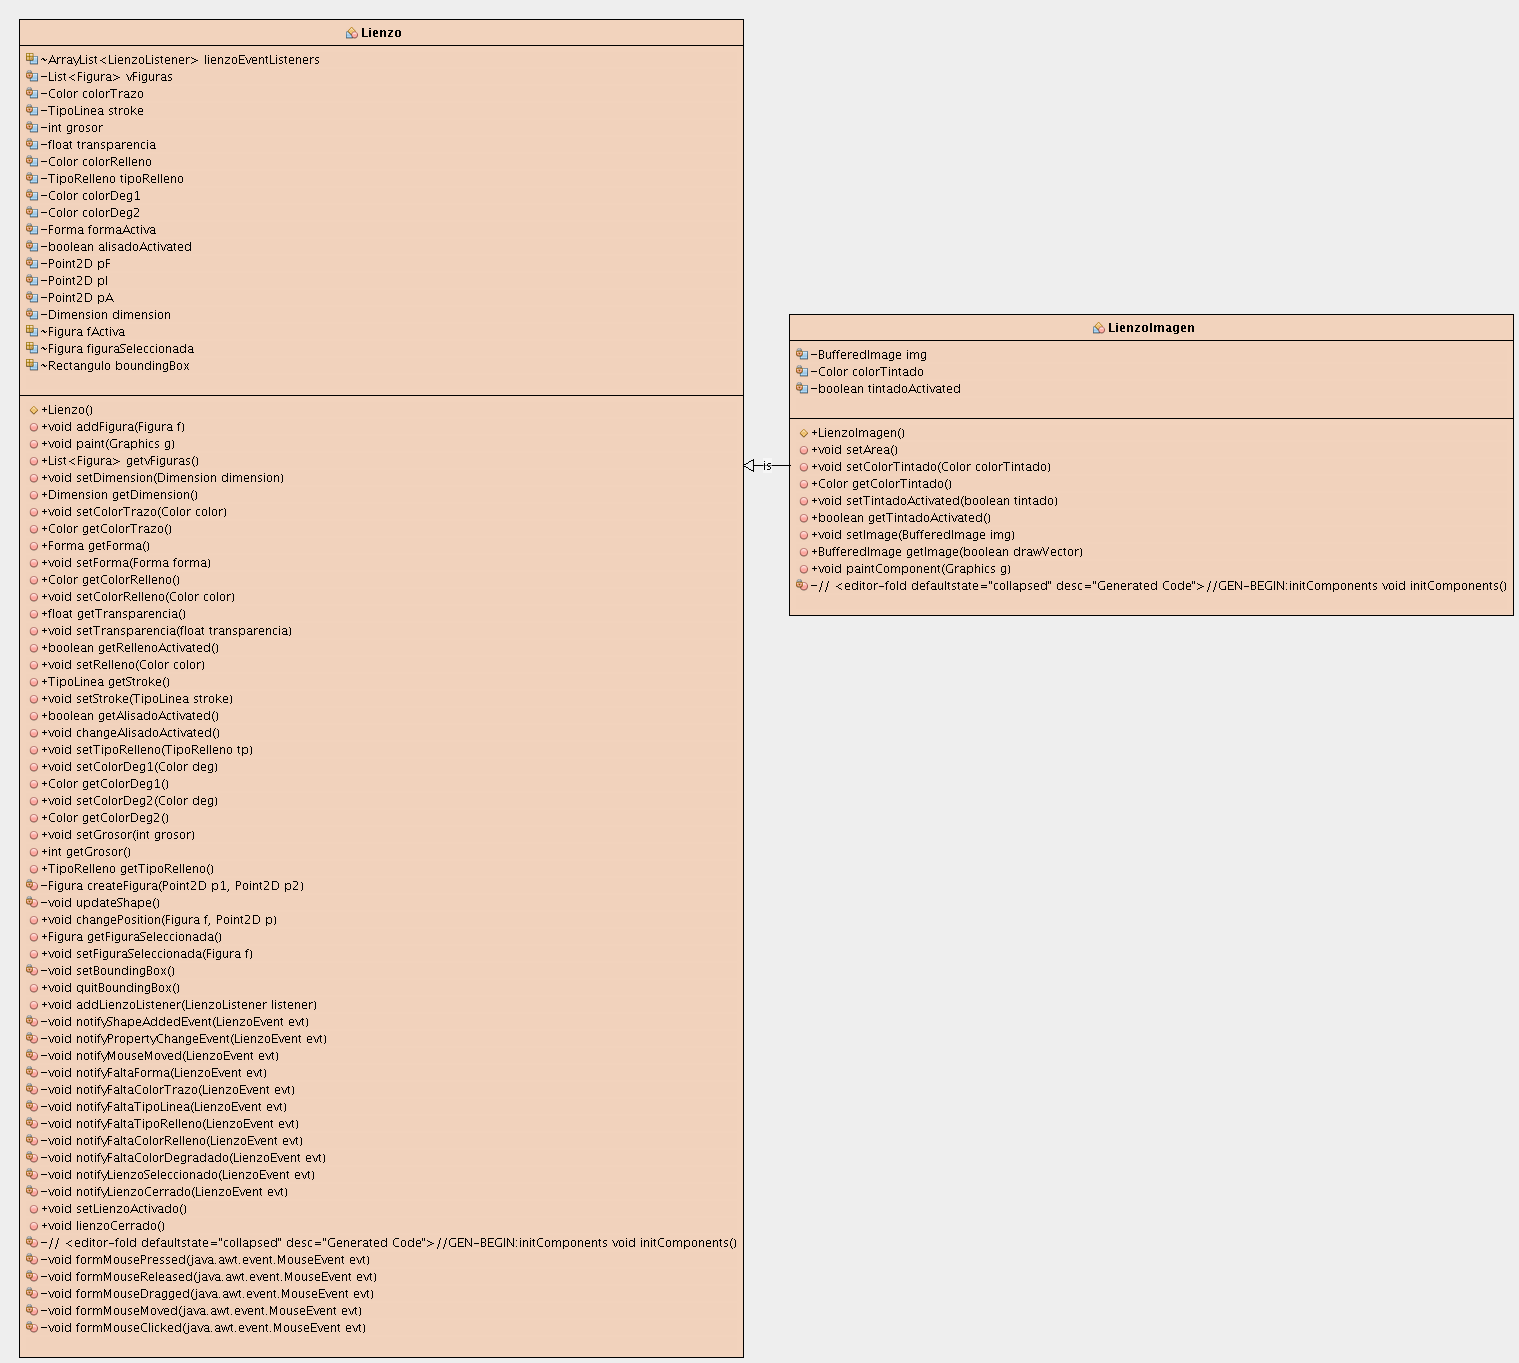
\includegraphics[width=0.9\textwidth]{diagramas/lienzo.png}
 \caption{Diagrama de clases \texttt{Lienzo}}
 \label{diseño}
 \end{figure}
\subsection{Ventanas internas}
Se definirá una clase \texttt{VentanaMultimedia} que heredará \texttt{JInternalFrame}. De esta clase derivarán diferentes ventanas en función del archivo multimedia que contengan.
\begin{itemize}
\item{\textbf{VentanaMultimediaImagen:} se encargará de almacenar el contenido multimedia de tipo imagen. Tendrá un objeto de clase \texttt{LienzoImagen}, que será un rectángulo en blanco en el caso de que sea creada por el usuario, y una imagen en el caso de que sea una imagen abierta. Contendrá también un elemento de tipo \texttt{JScrollPane} para el caso en que la ventana no pueda contener la imagen completa.\vskip0.3cm Se hará uso de las funciones \texttt{formInternalFrameActivated} y \texttt{formInternalFrameDeactivated} para actualizar los atributos de la barra de herramientas cuando se seleccione una ventana imagen, así como para activar/desactivar los atributos de procesamiento de imágenes.}
\item{\textbf{VentanaMultimediaCamara:} se encargará de almacenar las imágenes que pueden verse desde la WebCam así como las funciones encargadas de gestionar este contenido.Se hará uso de la función \texttt{formInternalFrameClosing} para cerrar la cámara cuando se cierre la ventana que muestra la imagen de la Webcam.}
\item{\textbf{VentanaMultimediaVLCPlayer:} se encargará de almacenar vídeos así como las funciones encargadas de gestionar este contenido.}
\end{itemize}
\vskip0.3cm
\begin{figure}
 \centering
  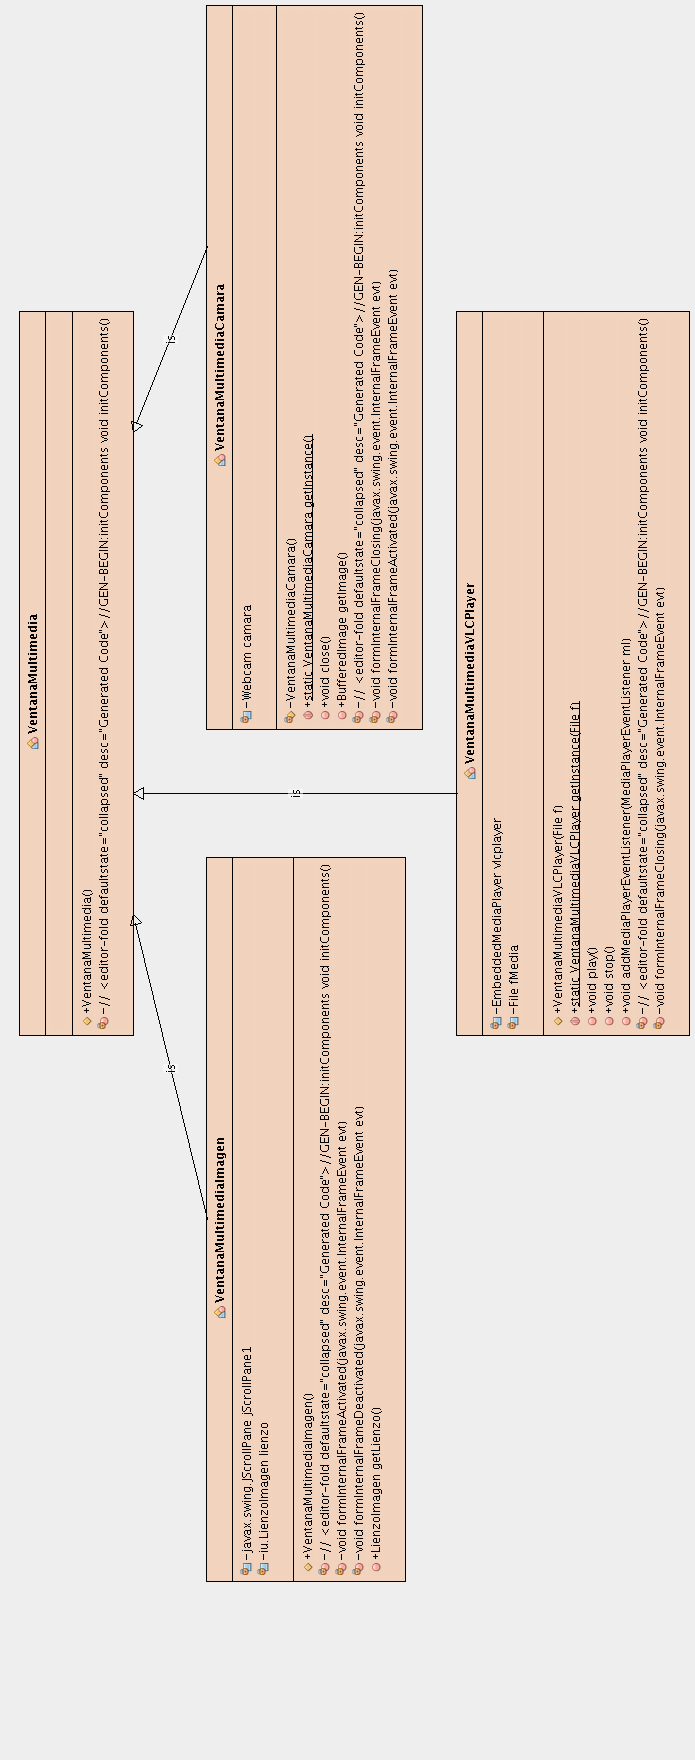
\includegraphics[width=0.6\textwidth]{diagramas/ventanaMultimedia.png}
 \caption{Diagrama de clases \texttt{VentanMultimedia}}
 \label{diseño}
 \end{figure}

\subsection{Figura}
Se definirá la clase abstracta \texttt{Figura}. Esta clase almacenará los atributos de la figura a crear. Las clases \texttt{FiguraRellenable} y \texttt{FiguraLineal} heredarán de \texttt{Figura}. Aunque en este caso no hay más de una figura lineal, este esquema permite que en posteriores versiones se añadan curvas u otro tipo de figuras lineales. \vskip0.3cm
De \texttt{FiguraRellenable} heredarán \texttt{Rectangulo},\texttt{Elipse} y \texttt{RectanguloRedondeado}. De \texttt{FiguraLineal} heredará la clase \texttt{Linea}. Cada una de estas clases tendrá asociado un objeto \texttt{Shape}, además de los atributos de las clases de las que hereda:\begin{itemize}
\item{Línea: \texttt{Line2D}.}
\item{Rectángulo: \texttt{Rectangle2D}.}
\item{Rectángulo redondeado: \texttt{RoundRectangle2D}.}
\item{Elipse: \texttt{Ellipse2D}.}
\end{itemize}
\vskip0.3cm
Es esta jerarquía de clases la que permite que cada figura tenga sus propios atributos, así como la posibilidad de modificarlos \textbf{[RFD-8:10]}, llamando a los \textit{setters} del objeto.\vskip0.3cm
Esto permitirá consultar también los atributos de una figura, llamando a los distintos \textit{getters} para actualizar los atributos de la barra de figuras. Como \texttt{Figura} es una clase abstracta, debe tener como mínimo un método abstracto. Los métodos abstractos de la clase serán los siguientes:
\begin{itemize}
\item{\texttt{setLocation:} se encarga de cambiar la posición de una figura. En principio se pretendía aprovechar el método que proporcionaba \texttt{Graphics}, pero se ha optado por implementarlo en cada clase de forma manual, ya que para \texttt{Rectangle2D} y \texttt{Ellipse2D} no está disponible el uso de esta función.}
\item{\texttt{updateShape:} actualiza una figura a partir de los puntos de inicio y final.}
\end{itemize}
Más detalles acerca de los atributos asociados a la clase \texttt{Figura}, así como métodos para utilizarlos pueden consultarse en el diagrama.
\vskip0.3cm
\begin{figure}
 \centering
  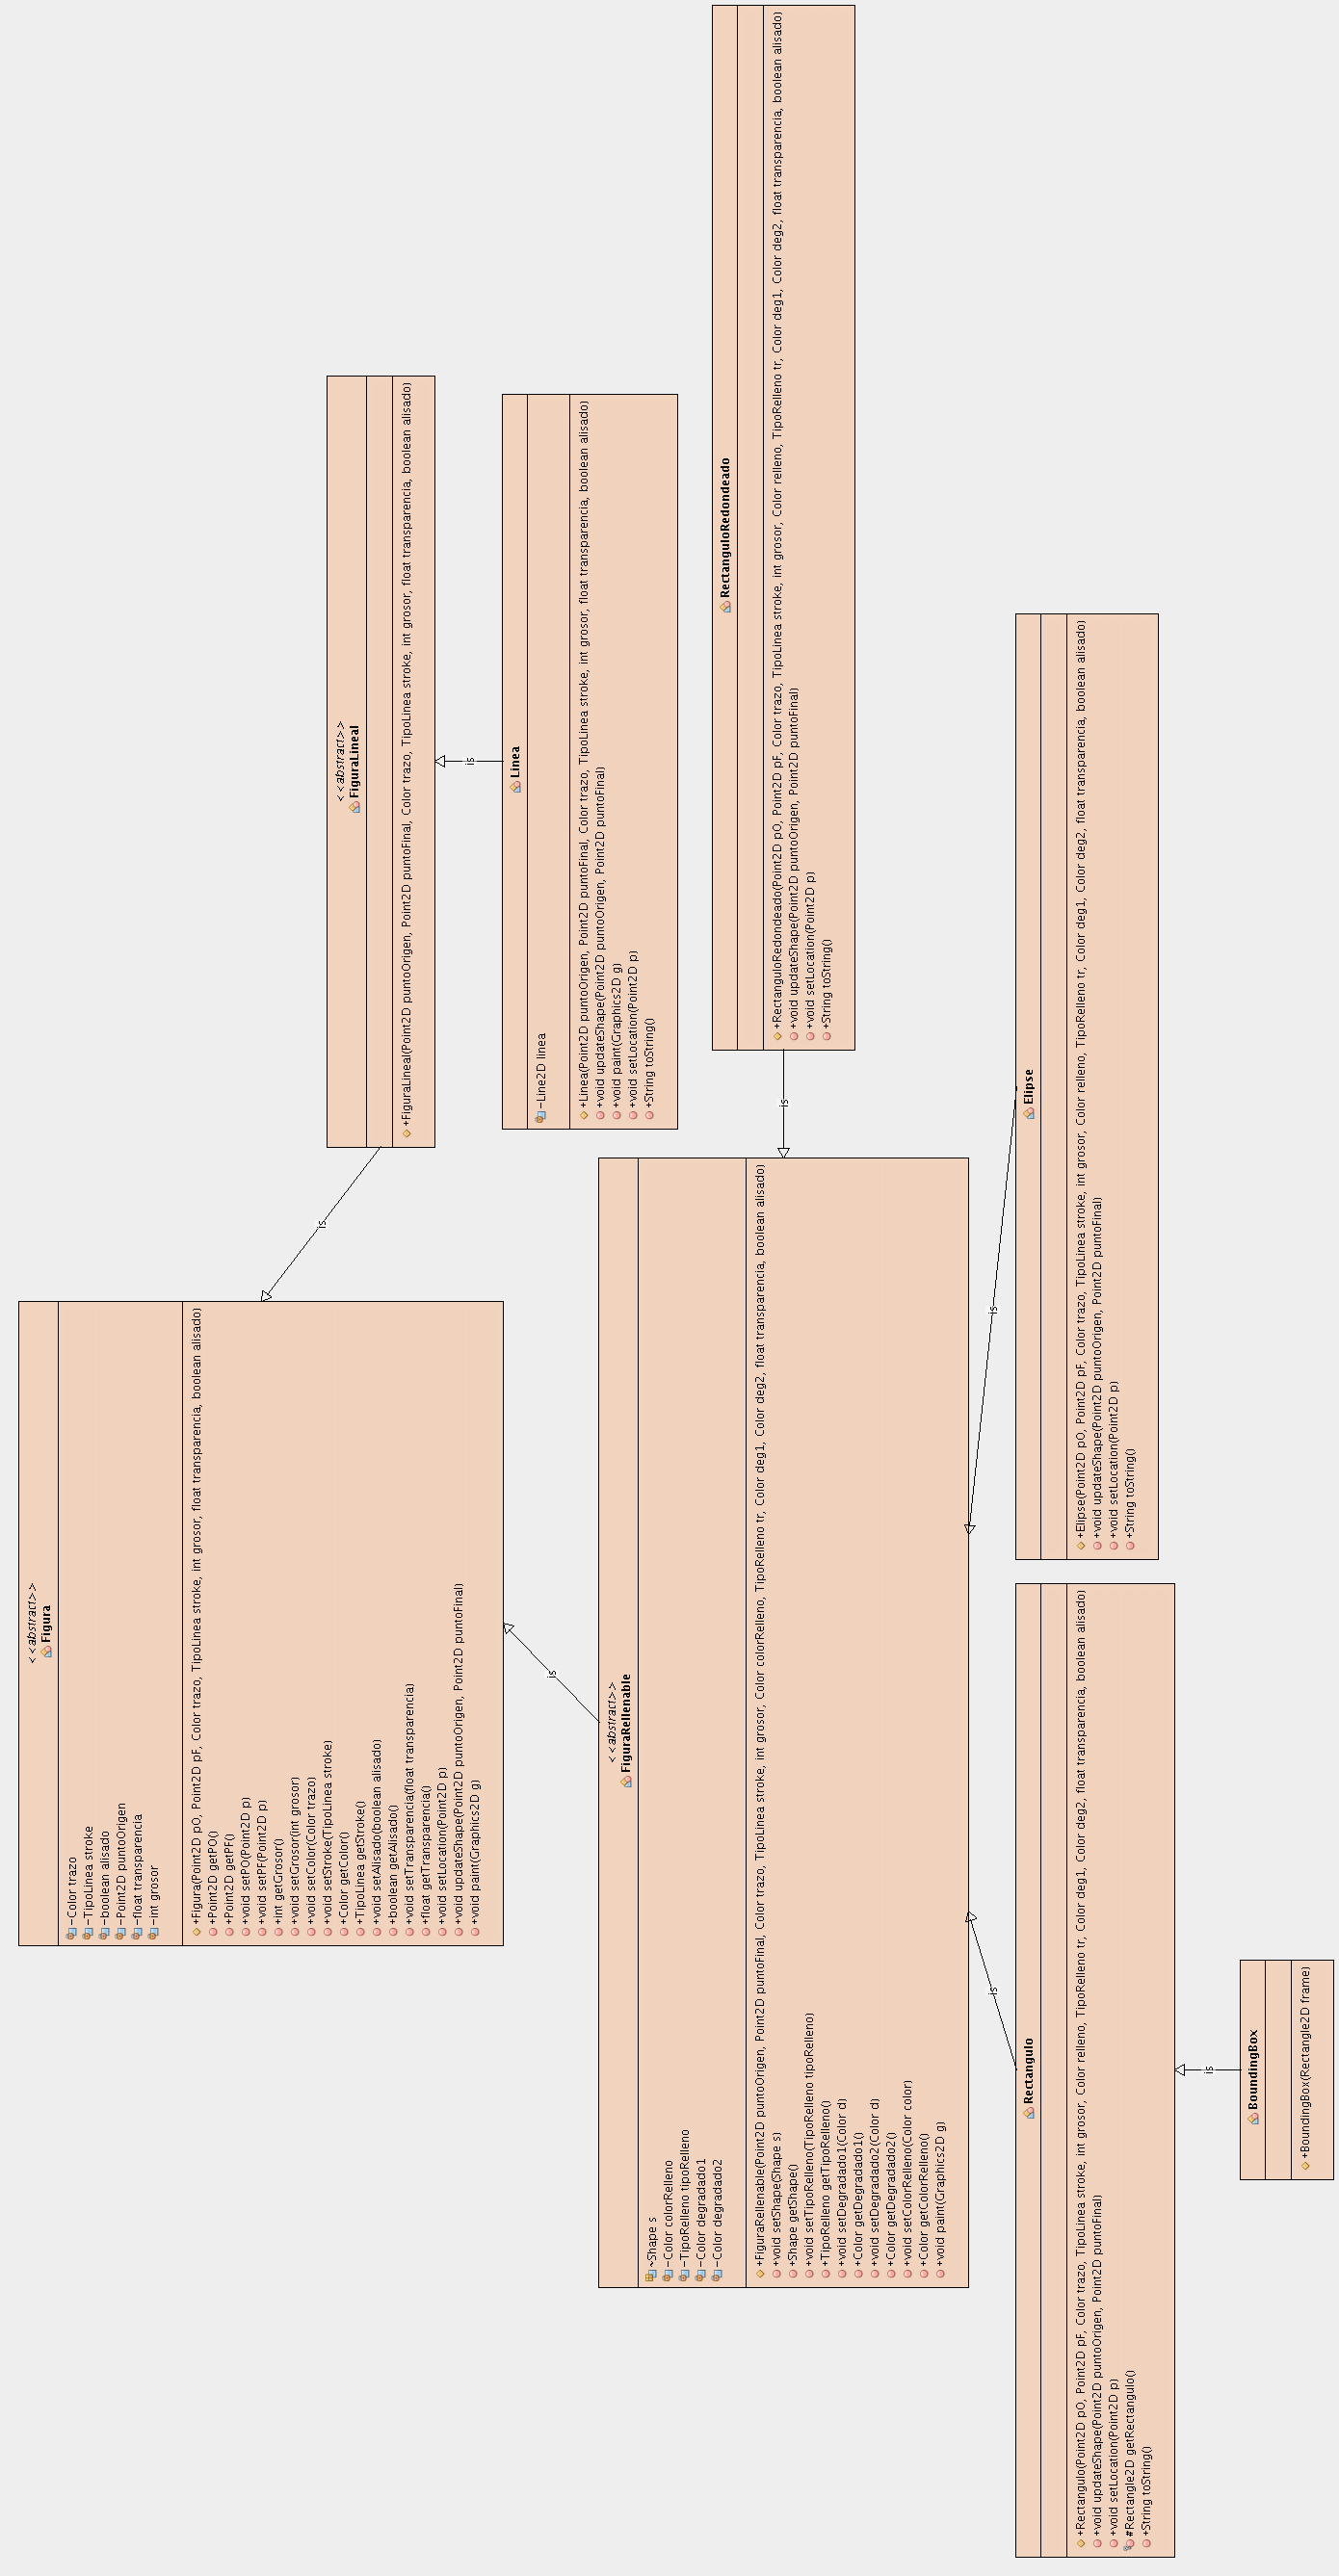
\includegraphics[width=0.8\textwidth]{diagramas/figura.png}
 \caption{Diagrama de clases \texttt{Figura}}
 \label{diseño}
 \end{figure}

\subsection{Gestión de eventos}
Se hará uso de las funciones de gestión de eventos que ofrece \textit{Java} para los botones, \texttt{ActionEvent}, \texttt{FocusGained}, \texttt{FocusLost},... Sin embargo, es necesario implementar las funciones para la gestión de eventos en el lienzo, de forma que podamos establecer una comunicación entre lienzo y ventana principal.
\begin{itemize}
\item{\textbf{LienzoEvent:} representa un evento lanzado por un objeto \texttt{Lienzo}. Heredará de la clase \texttt{EventObject} y tendrá asociados gran parte de los atributos de la clase \texttt{Lienzo}.}
\item{\textbf{LienzoListener:} interfaz que hereda de \texttt{EventListener}. Definirá las distintas causas que generan el evento. Por ejemplo, el movimiento del ratón.}
\item{\textbf{LienzoAdapter:} clase que implementa la interfaz \texttt{LienzoListener} y de la que heredará \texttt{MiManejadorLienzo}, de ahí el nombre de \textit{Adapter}.}
\item{\textbf{MiManejadorLienzo:} hereda de \texttt{LienzoListener}. Será necesario asociar un manejador a cada uno de los lienzos. Esta clase estará implementada dentro de \texttt{VentanaPrincipal} y será la que modificará los elementos \texttt{Swing} cuando el lienzo lance un evento. Por ejemplo: si se añade una figura en el lienzo, la barra de estado de la ventana principal indicará que se ha añadido dicha figura \textbf{[RFD-11,12,16]}.}
\end{itemize}

\vskip0.3cm
\begin{figure}
 \centering
  \includegraphics[width=1.1\textwidth]{diagramas/LienzoEvent.png}
 \caption{Diagrama de clases \texttt{LienzoEvent}, \texttt{LienzoListener}, \texttt{LienzoAdapter} y \texttt{MiManejadorLienzo}}
 \label{diseño}
 \end{figure}

\subsection{Procesamiento de imágenes (I)}
Este apartado expondrá algunos aspectos generales del procesamiento de imágenes.
\vskip0.3cm
Las imágenes serán del tipo \texttt{BufferedImage}, ofrecida por \texttt{Java} y se contará con la biblioteca \texttt{sm.image}, así como con las funciones ofrecidas por Java. En el lienzo existirá un método \texttt{getImage(boolean)}, que nos devolverá la imagen con las figuras que se han pintado sobre ella (si el parámetro es \texttt{true}) o solo la imagen en caso contrario. Como no es necesario que el procesamiento se aplique sobre las figuras dibujadas, en las funciones relacionadas con el procesamiento de imágenes el valor del parámetro será \texttt{false} \textbf{[RFPI-23]}.
\vskip0.3cm
Para duplicar una imagen \textbf{[RFPI-1]} será necesario crear una nueva \texttt{BufferedImage}, de forma que no se trate de una referencia a la imagen original. Si no fuese una copia, los cambios de una se aplicarían en la otra, de forma que no se estaría duplicando la imagen, sino abriendo la misma en una ventana diferente.\vskip0.3cm
De forma general, para crear una copia de una imagen se utilizarán los métodos \texttt{getColorModel}, \texttt{copyData} y \texttt{isAlphaPremultiplied} de la clase \texttt{BufferedImage}, y por tanto ofrecidas por \textit{Java}.
\vskip0.3cm
Para modificar el brillo de la imagen \textbf{[RFPI-2]} se utilizará la operación \texttt{RescaleOp}, disponible en la biblioteca de \textit{Java}. Se hará una copia de la imagen en el lienzo activo, ya que el cambio no será definitivo hasta que se desactive el deslizador (\texttt{FocusLost}).
\vskip0.3cm
Para aplicar los filtros de emborronamiento, enfoque y relieve \textbf{[RFPI-3,4,5]} en primer lugar será necesario crear una máscara en función del filtro, haciendo uso de la clase \texttt{KernelProducer} disponible en la biblioteca \texttt{sm.image} y, una vez creada la máscara, haciendo uso de \texttt{ConvolveOp} (\textit{Java}). Se utilizarán máscaras predefinidas:
\begin{itemize}
\item{\texttt{TYPE\_RELIEVE\_3x3} para el filtro de relieve.}
\item{\texttt{TYPE\_BINOMIAL\_3x3} para el filtro de emborronamiento.}
\item{\texttt{TYPE\_ENFOQUE\_3x3} para el filtro de enfoque.}
\end{itemize}
\vskip0.3cm
Para las operaciones de contraste, iluminado, oscurecido y negativo \textbf{[RFPI-6,7,8,10]}, al tratarse de una transformación sobre los niveles de color, se hará uso de \texttt{LookUpOp} (\textit{Java}). Para ello, se creará un objeto \texttt{LookUpTable} haciendo uso de \texttt{LookUpTableProducer} (\texttt{sm.image})  con un tipo determinado en función de la operación de la que se trate:
\begin{itemize}
\item{Contraste: \texttt{TYPE\_SFUNCION}.}
\item{Iluminado:\texttt{TYPE\_LOGARITHM}.}
\item{Oscurecido: \texttt{TYPE\_POWER}.}
\item{Negativo: \texttt{TYPE\_NEGATIVE}.}
\end{itemize}
Se utilizará este objeto \texttt{LookUpTable} para crear el objeto \texttt{LookUpOp}, y llamar al método \texttt{filter}. La imagen destino será la misma que la imagen fuente.  
\vskip0.3cm
Para la extracción de bandas \textbf{[RFPI-9]}, crearemos una imagen por cada una de las bandas de colores (roja, verde y azul), y las mostraremos en \texttt{VentanaMultimediaImagen} separadas en niveles de gris.
\begin{itemize}
\item{Se creará el modelo de color de la nueva imagen basada en niveles de gris haciendo uso de \texttt{CS\_GRAY}.}
\item{Se creará el nuevo raster a partir del de la imagen original.}
\item{Crear una nueva imagen haciendo uso del modelo de color y el raster de la banda correspondiente.}
\end{itemize}
\vskip0.3cm
La conversión a otros espacios de color \textbf{[RFPI-11]} se hará haciendo uso de \texttt{ColorConvertOp} y usando instancias de \texttt{ColorSpace}: \texttt{CS\_LINEAR\_RGB} para el espacio de color RGB, \texttt{CS\_PYCC} para YCC y \texttt{CS\_GRAY} para GREY.
\vskip0.3cm
Para el caso de el giro libre (en el que se incluye los casos particulares de $90º$, $180ª$, $270º$) y el escalado se utilizará la clase \texttt{AffineTransformOp} disponible en \textit{Java} \textbf{[RFPI-12,24]} . Para el giro se utilizará la función \texttt{getRotateInstance} y para el escalado \texttt{getScaleInstance}, usando los parámetros deseados (giro/escala). El giro tendrá asociado un elemento \texttt{Slider} para ajustar el ángulo al que se desea girar la imagen.
\vskip0.3cm
Para el filtro sepia y para la umbralización \textbf{[RFPI-18,16]} ha sido necesario crear clases propias, \texttt{SepiaOp} y \texttt{UmbralizacionOp}. Como en el siguiente apartado se hace un análisis más detallado de las clases de creación propia, aquí tan sólo se detalla la formulación matemática asociada a estos operadores.\vskip0.3cm
Se debe tener en cuenta que en la umbralización el valor \texttt{umbral} es la intensidad a partir de la cual el filtro realiza la transformación a color blanco. Por debajo de este umbral, la transformación será a color negro.
\vskip0.3cm
El nivel de umbralización se podrá determinar gracias a un \texttt{Slider} \textbf{[RFPI-17]}. 
\begin{lstlisting}[language=Java, caption=Filtro sepia, label=lst:graddesc]
		for(int x=0; x<src.getWidth(); x++){
            for(int y=0; y<src.getHeight(); y++){
                int sepiaR, sepiaG, sepiaB;
                int srcR, srcG, srcB;
                Color colorSrc = new Color(src.getRGB(x, y));
                Color colorDest;
                //color del pixel
                srcR = colorSrc.getRed();
                srcG = colorSrc.getGreen();
                srcB = colorSrc.getBlue();
                //convertirlo a sepia
                sepiaR = (int) Math.min(255, 0.393*srcR+0.769*srcG+0.189*srcB);
                sepiaG = (int) Math.min(255, 0.349*srcR+0.686*srcG+0.168*srcB);
                sepiaB = (int) Math.min(255, 0.272*srcR+0.534*srcG+0.131*srcB);
                
                colorDest = new Color(sepiaR, sepiaG, sepiaB);
                dest.setRGB(x, y, colorDest.getRGB());
            }
        }
\end{lstlisting}
\begin{lstlisting}[language=Java, caption=Filtro umbralización, label=lst:graddesc]
		for(int x=0; x<src.getWidth(); x++){
            for(int y=0; y<src.getHeight(); y++){
                int srcR, srcG, srcB;
                Color colorSrc = new Color(src.getRGB(x, y));
                //colores del pixel
                srcR = colorSrc.getRed();
                srcG = colorSrc.getGreen();
                srcB = colorSrc.getBlue();
                //intensidad como media de sus componentes
                int intensidad = (srcR + srcG + srcB)/3;
                if(intensidad>=umbral){
                    dest.setRGB(x, y, Color.WHITE.getRGB());
                }
                else{//intensidad < umbral
                    dest.setRGB(x, y, Color.BLACK.getRGB());
                }
            }
        }
\end{lstlisting}
\vskip0.3cm 
Para el tintado \textbf{[RFPI-13]}, así como para el ecualizado \textbf{[RFPI-15]}, se utilizarán los operadores \texttt{TintOp} y \texttt{EqualizationOp}, proporcionados por \texttt{sm.image}. Simplemente será necesario crear los objetos y llamar al método \texttt{filter}. En el caso del tintado hay tres elementos a tener en cuenta:
\begin{itemize}
\item{\texttt{JToggleButton} para activar/desactivar el tintado. Cuando se active el tintado, se habilitarán los siguientes dos elementos.}
\item{\texttt{JComboBox} con objetos de tipo \texttt{Color}. Permitirá escoger el tipo de color con el que se quiere tintar la imagen.}
\item{\texttt{Slider} para determinar el nivel de tintado\textbf{[RFPI-14]}.}
\end{itemize}
\subsection{Procesamiento de imágenes (II)}
En este apartado nos centraremos en las operaciones de diseño propio. Las operaciones que heredan de \texttt{BufferedImageOp} implementan operaciones punto a punto sobre la imagen, distinguiendo entre:
\begin{itemize}
\item{Operaciones píxel a píxel: para asignar el valor de una de las componentes del píxel se necesitará conocer el valor de otras componentes.}
\item{Operaciones componente a componente: no se necesitará conocer el valor de las otras componentes para asignar el valor de las componentes de un píxel.}
\end{itemize}
Para estas operaciones será necesario crear clases propias, en las que se sobrecargará el método \texttt{filter}. Este método tiene como parámetros \texttt{src}, \texttt{dest}, donde \texttt{src} es la imagen sobre la que se aplica el filtro y \texttt{det} la imagen en la que se guardará el resultado de aplicar el filtro.
\vskip0.3cm
Como queremos que el filtro se aplique sobre la misma imagen de origen, de forma que las operaciones se apliquen de forma concatenada, \texttt{src} y \texttt{dest} serán la misma imagen.
\vskip0.3cm
En el caso de que se defina una transformación sobre los niveles de color haciendo uso de \texttt{LookUpOp}, no será necesaria la creación de una clase propia, pero sí de una función que devuelva el objeto \texttt{LookUpTable} que defina la transformación deseada.
\vskip0.3cm
De la misma forma que en el caso anterior, una vez creado el objeto \texttt{LookUpOp}, se utilizará el método \texttt{filter}, donde \texttt{src} y \texttt{dest} serán la misma imagen, para que el filtro se aplique sobre la misma imagen. 
\subsubsection{Operador \textit{LookUpOp}}
Se definirá la función $f(x) = 255|cos(0.006x)|$, donde $0.06$ será la velocidad angular \textbf{[RFPI-22]}. De esta forma, será posible predecir el comportamiento de la función, ya que el coseno es una función periódica. Como se puede ver en la gráfica a continuación, predecir el comportamiento de la función sin reducir la velocidad angular sería imposible a simple vista.
\vskip0.3cm
\begin{figure}[H]
 \centering
  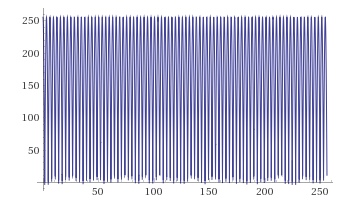
\includegraphics[width=0.4\textwidth]{imagenes/graficaCoseno2.png}
 \caption{Gráfica $f(x) = 255|cos(x)|$}
 \label{diseño}
 \end{figure}
Se escoge esa velocidad angular porque es lo suficientemente baja como para que no se complete un ciclo. A continuación se pinta la gráfica de $f(x)$. Se puede observar que se parece mucho a la función utilizada para invertir colores pero con $f(x)$ más altos. Se pintan las gráficas juntas para poder compararlas.
\vskip0.3cm
\begin{figure}[H]
 \centering
  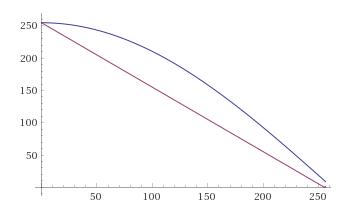
\includegraphics[width=0.5\textwidth]{imagenes/graficasjuntas.png}  
 \caption{Comparativa gráfica operación definida (azul) y gráfica operación invertir colores (morada)}
 \label{diseño}
 \end{figure}
 Por tanto el resultado esperado será una imagen similar a la que se obtendría invirtiendo los colores, con una mayor iluminación. A continuación puede comprobarse que el resultado obtenido es el esperado.
 \vskip0.3cm
\begin{figure}[H]
 \centering
  \includegraphics[width=0.3\textwidth]{imagenes/fry.jpg}
  
\includegraphics[width=0.3\textwidth]{imagenes/fryCos.jpg}
  
\includegraphics[width=0.3\textwidth]{imagenes/fryNegativo.jpg}
 \caption{Comparativa aplicación filtro cosinusoide y filtro negativo}
 \label{diseño}
 \end{figure}
\subsubsection{Componente a componente}
La función componente a componente modificará cada una de las componentes (R, G, B) de forma separada.\vskip0.3cm
En este caso se ha implementado un filtro violeta. Para aplicar un tono morado a la imagen, se tendrá en cuenta que la mezcla de rojo y azul es la que da lugar al morado. Por tanto, para obtener el efecto deseado se reducirá el valor de la componente verde y se aumentará el valor de la componente roja y azul \textbf{[RFPI-19]}.
\vskip0.3cm
Además, como se ha aumentado el valor de las componentes de forma significativa, habrá un aumento de la luminosidad en estos colores y de la intensidad de la imagen en general.
\vskip0.3cm
\begin{lstlisting}[language=Java, caption=Operación componente a componente, label=lst:graddesc]
for(int x=0; x<src.getWidth(); x++){
    for(int y=0; y<src.getHeight(); y++){
        int destR, destG, destB;
        int srcR, srcG, srcB;
        Color colorSrc = new Color(src.getRGB(x, y));
        Color colorDest;
        //color del pixel
        srcR = colorSrc.getRed();
        srcG = colorSrc.getGreen();
        srcB = colorSrc.getBlue();
        //operacion componente a componente
        destR = (int) Math.min(255,1.3*srcR);
        destG = (int) Math.min(255,0.2*srcG);
        destB = (int) Math.min(255,1.5*srcB);
                
        colorDest = new Color(destR, destG, destB);
        dest.setRGB(x, y, colorDest.getRGB());
     }
}
\end{lstlisting}
El resultado de aplicar el filtro puede verse a continuación. Como se puede ver, se obtiene el resultado deseado.
\vskip0.3cm
\begin{figure}[H]
 \centering
  
\includegraphics[width=0.3\textwidth]{imagenes/Fry.jpg}
  
\includegraphics[width=0.3\textwidth]{imagenes/fryVioleta.jpg}
 \caption{Aplicación filtro violeta sobre \texttt{Fry.jpg}}
 \label{diseño}
 \end{figure}

\vskip0.3cm
\begin{figure}[H]
 \centering
  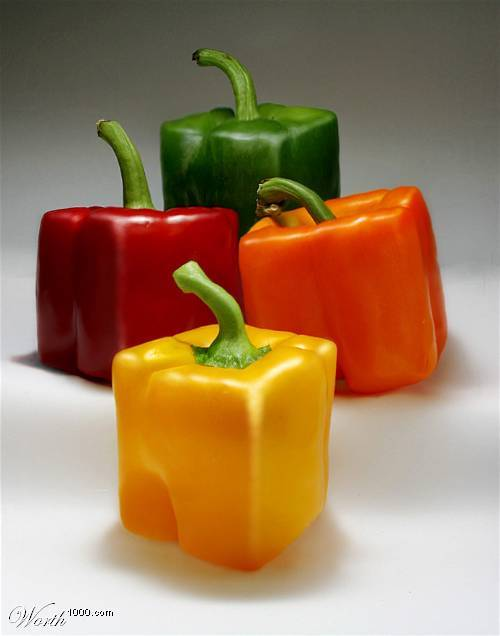
\includegraphics[width=0.3\textwidth]{imagenes/pimientos.jpg}
  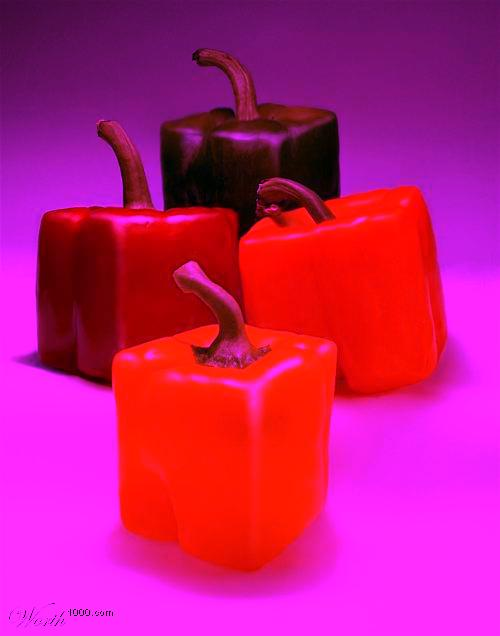
\includegraphics[width=0.3\textwidth]{imagenes/pimientosVioleta.jpg}
 \caption{Aplicación filtro violeta}
 \label{diseño}
 \end{figure} 
 
\subsubsection{Primera operación píxel a píxel}
La función píxel a píxel modificará cada componente teniendo en cuenta los demás componentes, de forma que el valor de cada componente podrá ser una combinación de las otras.
\vskip0.3cm
La operación implementada en este caso es una especie de "filtro rojizo", aunque no llega a serlo como tal. El valor del color rojo se conservará tal y como está, mientras que los valores verde y azul serán una media de los otros tres, por lo que aquellos píxeles en los que estos valores sean predominantes tendrán un color grisáceao \textbf{[RFPI-21]}.
\vskip0.3cm
Se espera que en la primera aplicación del filtro, la imagen tomará este color rojizo-anaranjado, pues habrá sido la única componente que habrá mantenido su valor. Sin embargo, al estar esta componente presente en la media que asigna los valores verde y azul, a través de las sucesivas aplicaciones del filtro estos dos valores convergerán al valor de la componente roja, convirtiéndose en un filtro blanco y negro.
\begin{lstlisting}[language=Java, caption=Operación pixel a pixel, label=lst:graddesc]
for(int x=0; x<src.getWidth(); x++){
    for(int y=0; y<src.getHeight(); y++){
        int destR, destG, destB;
        int srcR, srcG, srcB;
        Color colorSrc = new Color(src.getRGB(x, y));
        Color colorDest;
        //color del pixel
        srcR = colorSrc.getRed();
        srcG = colorSrc.getGreen();
        srcB = colorSrc.getBlue();
        //operacion pixel a pixel
        destR = srcR;
        destG = Math.min(255,(srcR+srcG+srcB)/3);
        destB = Math.min(255,(srcR+srcG+srcB)/3);
                
        colorDest = new Color(destR, destG, destB);
        dest.setRGB(x, y, colorDest.getRGB());
    }
}
\end{lstlisting}
\vskip0.3cm
\begin{figure}[H]
 \centering
 
\includegraphics[width=0.3\textwidth]{imagenes/Fry.jpg}
  
\includegraphics[width=0.3\textwidth]{imagenes/fryMedia1.jpg}
  \vskip0.1cm
  
\includegraphics[width=0.3\textwidth]{imagenes/fryMedia2.jpg}
  
\includegraphics[width=0.3\textwidth]{imagenes/fryMedia3.jpg}
 \caption{Aplicaciones sucesivas operación píxel a píxel (I)}
 \label{diseño}
 \end{figure} 

\vskip0.3cm
\begin{figure}[H]
 \centering
 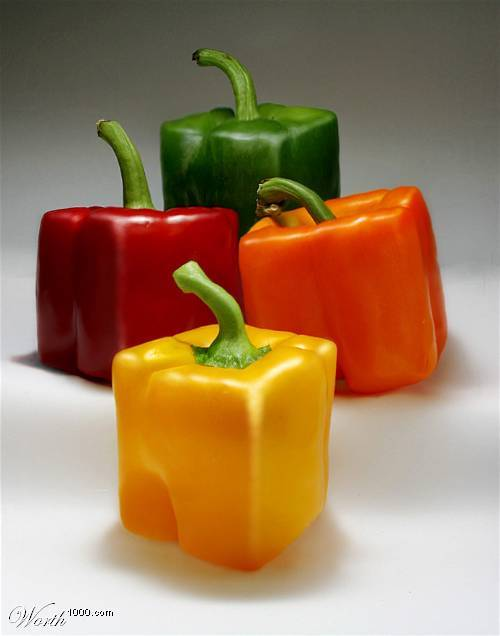
\includegraphics[width=0.3\textwidth]{imagenes/pimientos.jpg}
  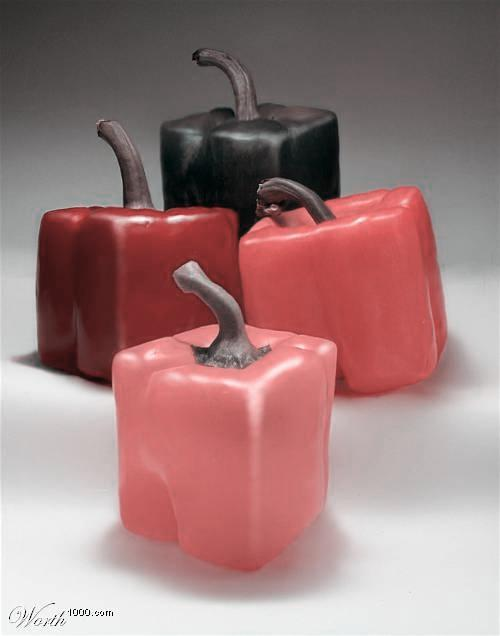
\includegraphics[width=0.3\textwidth]{imagenes/pimientosMedia1.jpg}
  \vskip0.1cm
  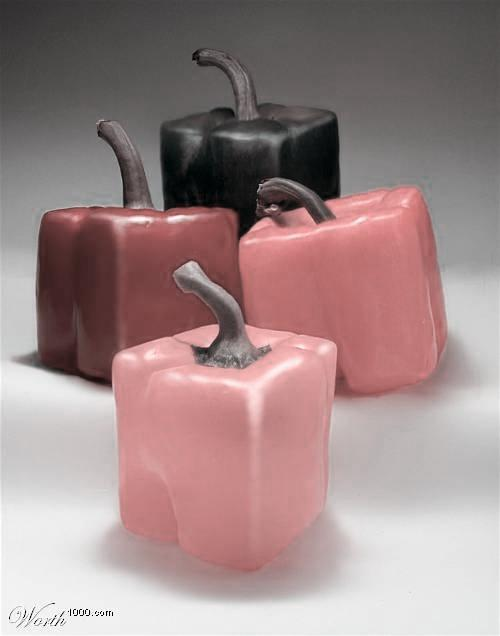
\includegraphics[width=0.3\textwidth]{imagenes/pimientosMedia2.jpg}
  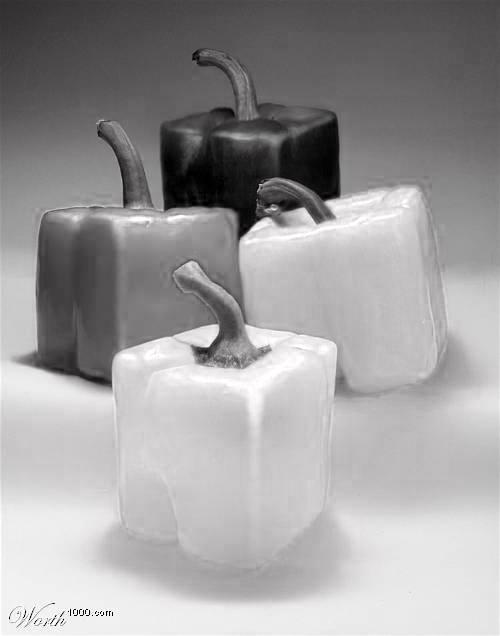
\includegraphics[width=0.3\textwidth]{imagenes/pimientosMedia3.jpg}
 \caption{Aplicaciones sucesivas operación píxel a píxel (II)}
 \label{diseño}
 \end{figure} 

\subsubsection{Segunda operación píxel a píxel}
Esta función es una variante de la primera, en la que se pretende que el filtro anterior no sea a través de las aplicaciones un filtro blanco y negro, sino un filtro que potencie el color rojo. Para ello, simplemente se elimina la componente roja de la media, de forma que los valores azules y verde no convergerán al valor de la componente roja \textbf{[RFPI-20]}.
\vskip0.3cm
\begin{lstlisting}[language=Java, caption=Operación pixel a pixel, label=lst:graddesc]
for(int x=0; x<src.getWidth(); x++){
    for(int y=0; y<src.getHeight(); y++){
        int destR, destG, destB;
        int srcR, srcG, srcB;
        Color colorSrc = new Color(src.getRGB(x, y));
        Color colorDest;
        //color del pixel
        srcR = colorSrc.getRed();
        srcG = colorSrc.getGreen();
        srcB = colorSrc.getBlue();
        //operacion pixel a pixel
        destR = srcR;
        destG = (srcG+srcB)/2;
        destB = (srcG+srcB)/2;
                
        colorDest = new Color(destR, destG, destB);
        dest.setRGB(x, y, colorDest.getRGB());
    }
}
\end{lstlisting}
A continuación pueden verse ejemplos de la aplicación de este filtro, que ofrece el resultado esperado.
\vskip0.3cm
\begin{figure}[H]
 \centering
 
\includegraphics[width=0.3\textwidth]{imagenes/Fry.jpg}
  
\includegraphics[width=0.3\textwidth]{imagenes/fryRojido.jpg}
  \vskip0.3cm
  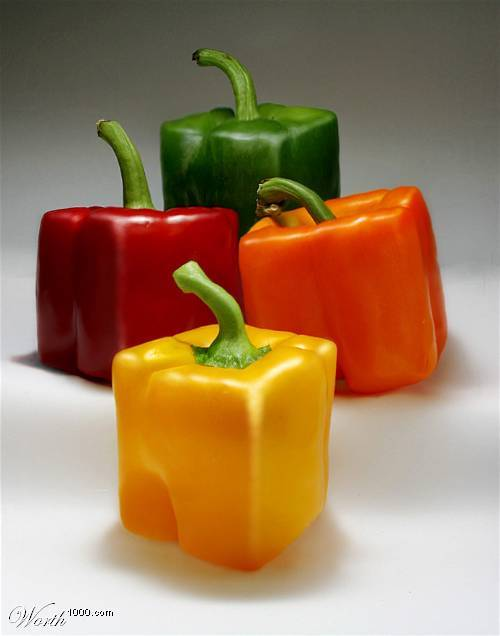
\includegraphics[width=0.3\textwidth]{imagenes/pimientos.jpg}
  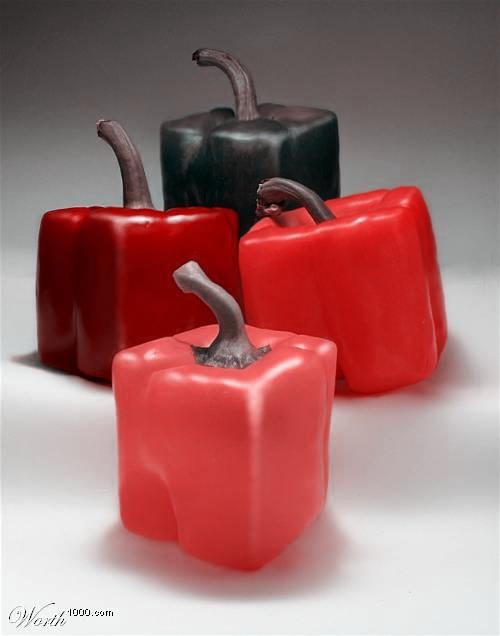
\includegraphics[width=0.3\textwidth]{imagenes/pimientoRojizo.jpg}
 \caption{Aplicación filtro rojizo}
 \label{diseño}
 \end{figure}
 
\subsection{Sonido}
Se hará uso del paquete \texttt{sm.sound}, que incluirá dos módulos:
\begin{itemize}
\item{\texttt{SMPlayer:} se harán uso de las funciones \texttt{play()}, \texttt{stop()} \textbf{[RFS-1,4]}.}
\item{\texttt{SMRecorder:} se harán uso de las funciones \texttt{record()}, \texttt{stop()} \textbf{[RFS-2,3]}.}
\end{itemize}
Cuando se inicialice un \texttt{player} o un \texttt{recorder} será necesario asociar un manejador que implementa \texttt{LineListener} haciendo uso de la función \texttt{addLineListener} que nos permita habilitar/deshabilitar los botones relacionados con el sonido en función de las acciones que realicemos. Por ejemplo, si se inicia la grabación, se debe deshabilitar el botón de inicio de grabación y habilitar el de detención \textbf{[RNF-2]}.
\subsection{Vídeo}
Para usar la Webcam se hará uso de la biblioteca \texttt{github.sarxos.webcam.Webcam}. Para abrir la Webcam se usará el método \texttt{getInstance()}, que creará una instancia de \texttt{Webcam} e inicializará la \texttt{VentanaMultimediaCamara} que contendrá las imágenes que se obtendrán desde la cámara \textbf{[RFV-1]}. Para hacer una captura de pantalla se utilizará el método \texttt{getImagen()}, que devolverá una objeto del tipo \texttt{BufferedImage} \textbf{[RFV-2]}.
\vskip0.3cm
Se hará uso de los métodos y las ventajas que ofrece la biblioteca \texttt{VLCj}, que permite acceder a formatos y códecs actualizados \textbf{[RFV-3,4]}. Se asociará un manejador para poder gestionar los eventos relacionados con el vídeo. La clase manejadora de eventos implementará \texttt{MediaPlayerEventAdapter} y, al igual que el manejador de sonido, habilitará/deshabilitará los botones relacionados con el vídeo \textbf{[RFV-2]}\textbf{[RNF-2]}. 
%%%%%%%%%%%%%%%%%%%%% IMPLEMENTACION %%%%%%%%%%%%%%%%%%%
\clearpage
\section{Implementación}
A continuación se muestra el resultado de la implementación de las clases diseñadas en el apartado anterior.
\subsection{Ventana principal}
\vskip0.3cm
\begin{figure}[H]
 \centering
  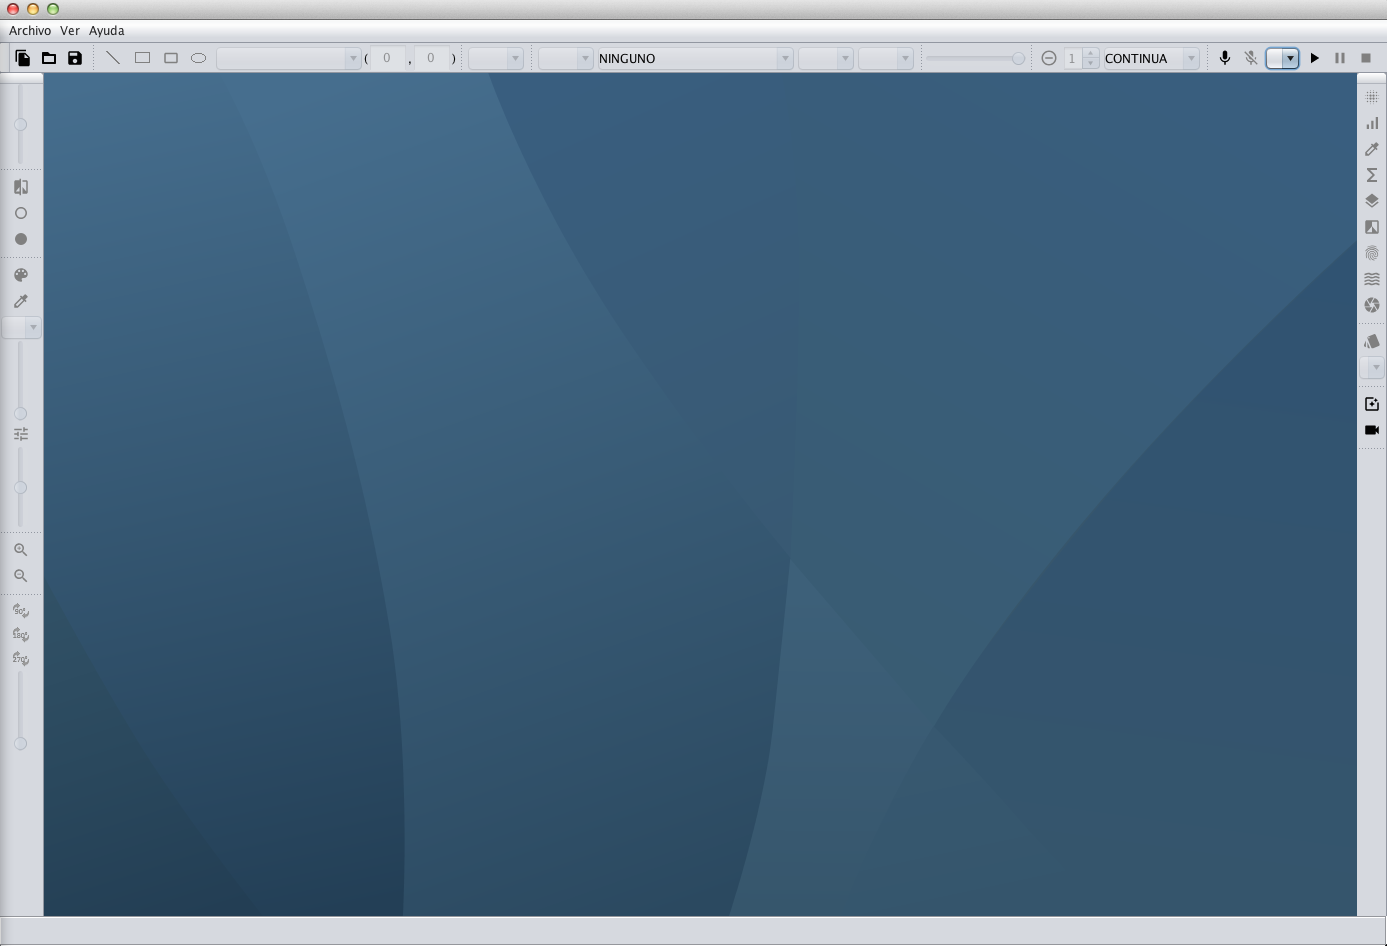
\includegraphics[width=0.8\textwidth]{graficos/ventanaPrincipal.png}
 \caption{Vista \texttt{VentanaPrincipal}}
 \label{diseño}
 \end{figure}
 
\subsection{VentanaMultimediaImagen}
\vskip0.3cm
\begin{figure}[H]
 \centering
  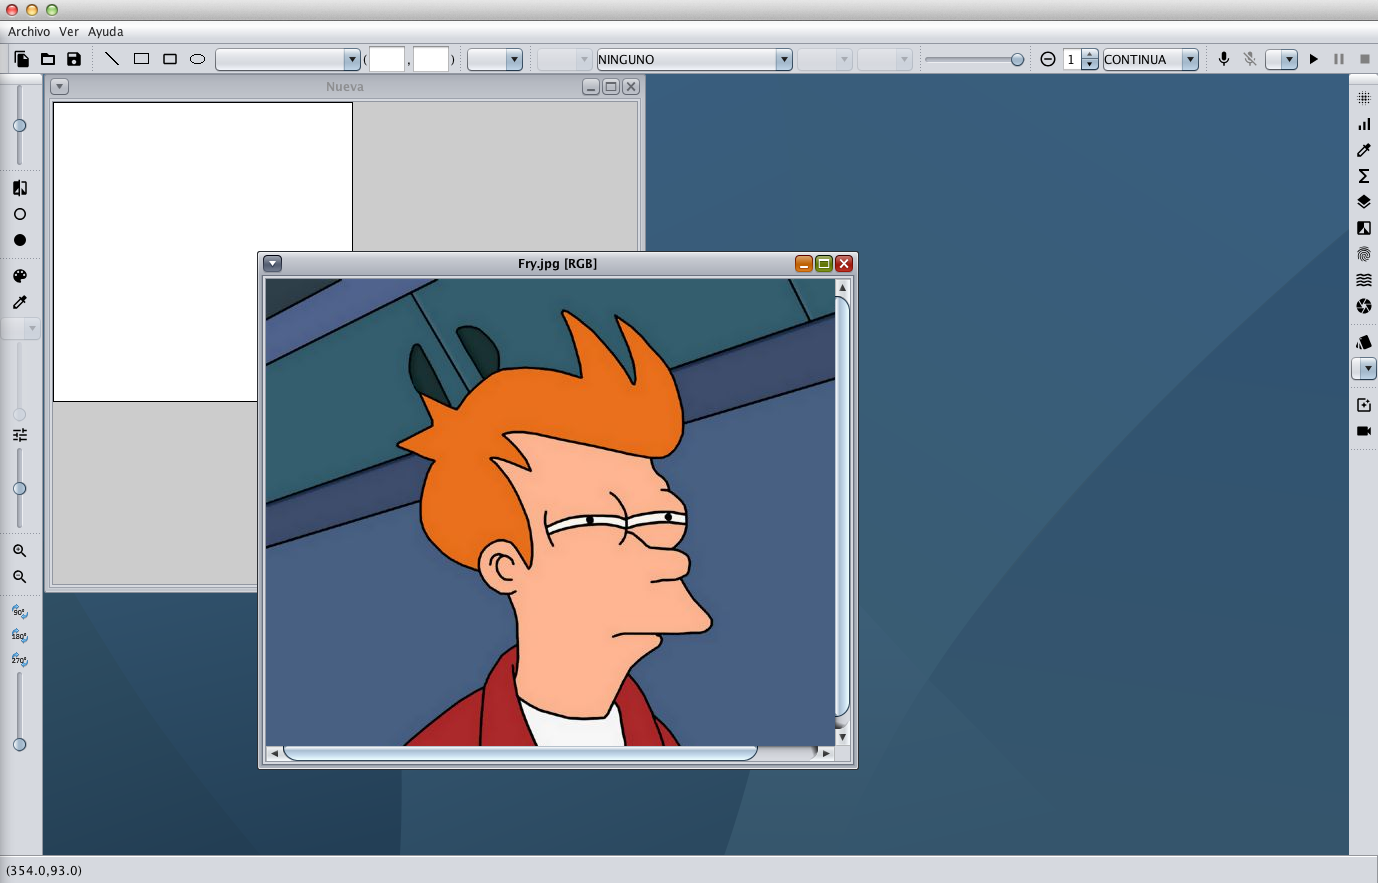
\includegraphics[width=0.7\textwidth]{graficos/ventanaImagen.jpg}
 \caption{Vista \texttt{VentanaMultimediaImagen}}
 \label{diseño}
 \end{figure}

\subsection{VentanaMultimediaCamara}
 
\vskip0.3cm
\begin{figure}[H]
 \centering
  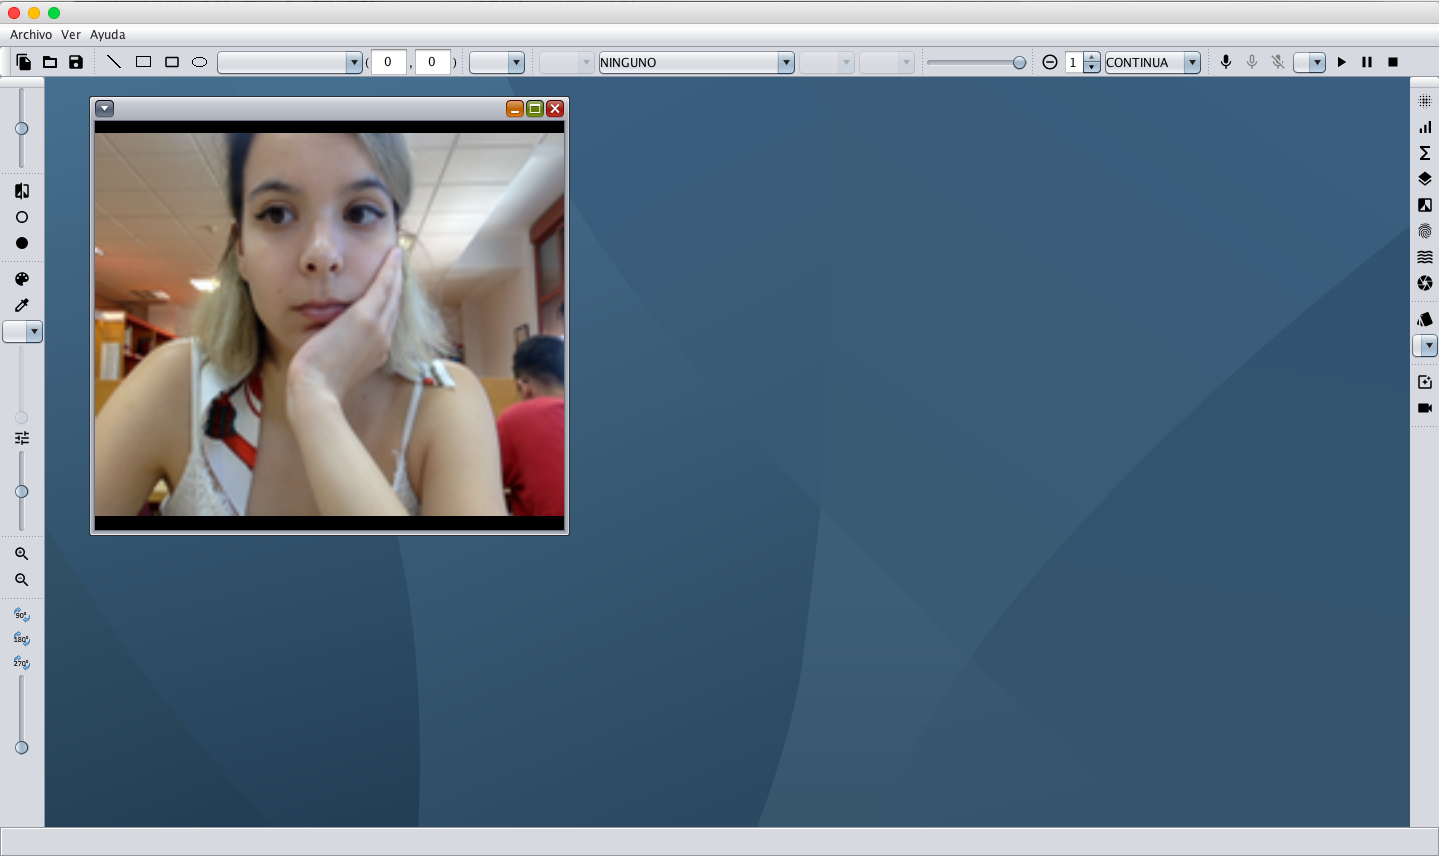
\includegraphics[width=0.8\textwidth]{video/webcam.jpg}
 \caption{Vista \texttt{VentanaMultimediaCamara}}
 \label{diseño}
 \end{figure}

\subsection{VentanaMultimediaVLCPlayer} 
 No se ha podido obtener la vista. He tenido problemas para cargar las librerías en mi ordenador con sistema operativo \textit{MacOS}, por lo que intenté probar el programa en un ordenador con un sistema operativo distinto. Se hizo la prueba en un ordenador \textit{Windows} y la reproducción funcionaba, aunque sólo el audio: la terminal mostraba un error relacionado con la tarjeta gráfica.
 %%%%%%%%%%%%%%%%% VALIDACION
\clearpage
\section{Validación}
En este apartado se comprobará que el programa implementado en base a la solución propuesta cumple con lo esperado.
\subsection{Generales}
\subsubsection{Crear una nueva imagen}
A la hora de crear una nueva imagen, el usuario podrá escoger las dimensiones del área de dibujo a través de ventanas emergentes. Para crear un archivo se puede tanto pulsar el botón habilitado para ello como acceder desde el menú \textbf{Archivo}.
\vskip0.3cm
\begin{figure}[H]
 \centering
  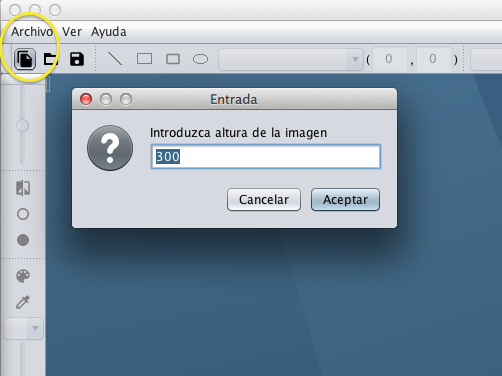
\includegraphics[width=0.4\textwidth]{generales/altura.png}
 \caption{Diálogo para escoger las dimensiones de la nueva imagen}
 \label{diseño}
 \end{figure}
\begin{figure}[H]
 \centering
  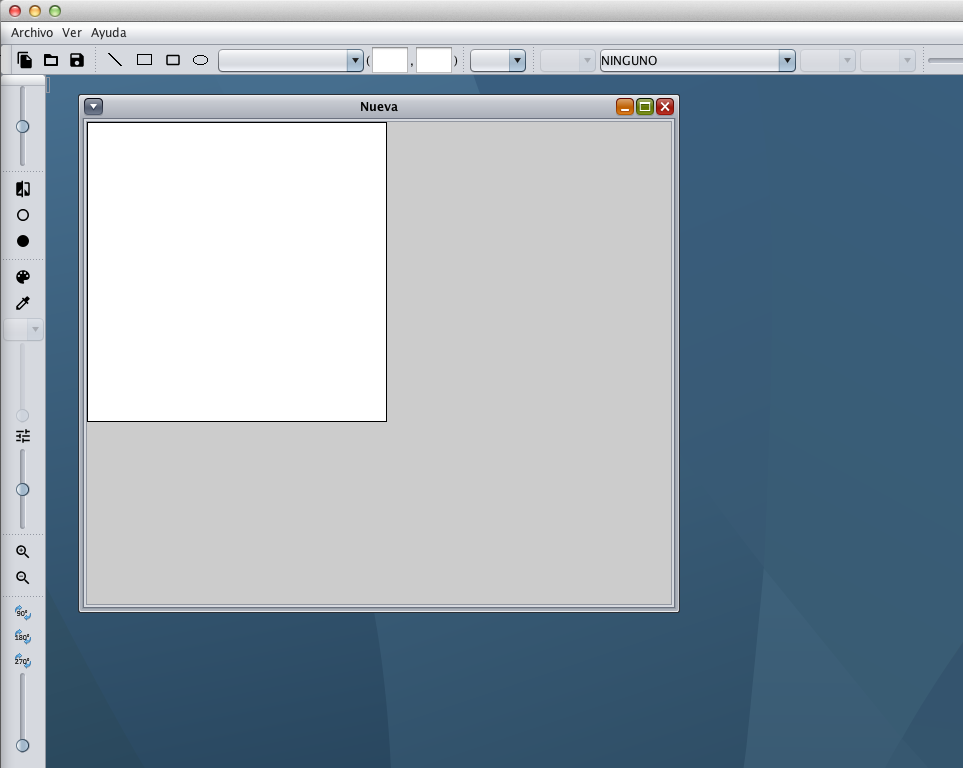
\includegraphics[width=0.4\textwidth]{generales/nuevo.png}
 \caption{Crear nuevo archivo}
 \label{diseño}
 \end{figure}
\subsubsection{Abrir un nuevo archivo}
Para abrir un archivo se puede tanto pulsar el botón habilitado para ello como acceder desde el menú \textbf{Archivo}. Si se abre un archivo de sonido, se añadirá a la lista desplegable de audios, mientras que si se abre una imagen o un vídeo, se abrirá una ventana multimedia que contendrá el archivo deseado.
\vskip0.3cm
\begin{figure}[H]
 \centering
  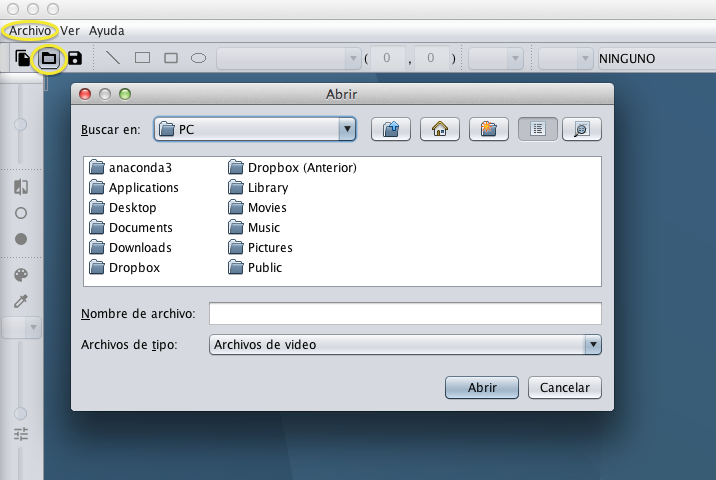
\includegraphics[width=0.41\textwidth]{generales/abrirImagen1.png}
  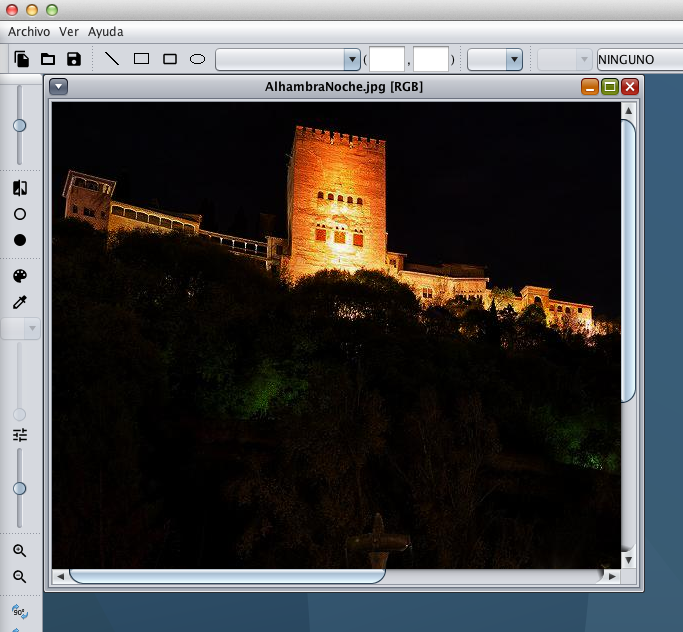
\includegraphics[width=0.3\textwidth]{generales/abrirImagen2.png}
 \caption{Abrir una imagen}
 \label{diseño}
 \end{figure}
 \vskip0.3cm
\begin{figure}[H]
 \centering
  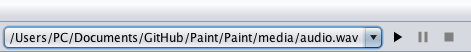
\includegraphics[width=0.5\textwidth]{sonido/archivoAbierto.png}
 \caption{Abrir archivo de sonido}
 \label{diseño}
 \end{figure}
\subsubsection{Guardar un archivo}
Para guardar un archivo se puede tanto pulsar el botón habilitado para ello como acceder desde el menú \textbf{Archivo}.
\vskip0.3cm
\begin{figure}[H]
 \centering
  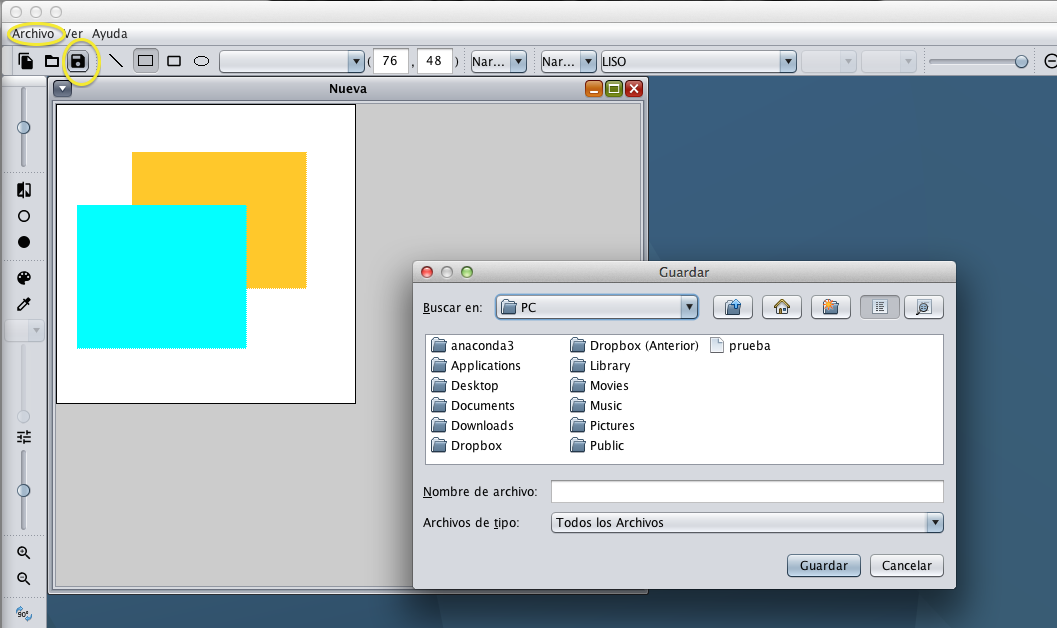
\includegraphics[width=0.4\textwidth]{generales/guardar.png}
  
\includegraphics[width=0.25\textwidth]{generales/prueba.png}
 \caption{Guardar una imagen}
 \label{diseño}
 \end{figure}
\subsubsection{Ocultar/mostrar barras de herramientas}
Será posible ocultar/mostrar las barras de herramientas y de estado haciendo haciendo uso de las checkboxs disponibles en el menú \textbf{Ver}.
\vskip0.3cm
\begin{figure}[H]
 \centering
  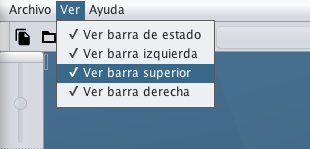
\includegraphics[width=0.3\textwidth]{generales/ocultarBarras1.png}
  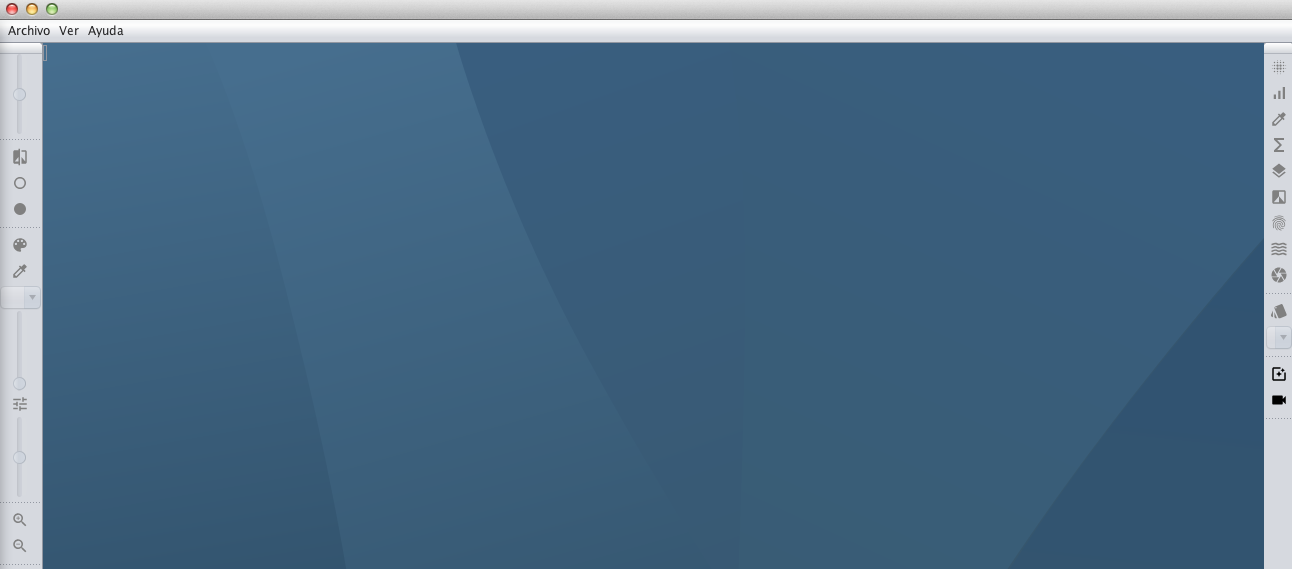
\includegraphics[width=0.3\textwidth]{generales/ocultarBarras2.png}
 \caption{Ocultar barras de herramientas}
 \label{diseño}
 \end{figure}
\subsubsection{Acerca de}
El menú \textbf{Ayuda} contendrá la opción \textbf{Acerca de} que lanzará el diálogo con la información del programa.
\vskip0.3cm
\begin{figure}[H]
 \centering
  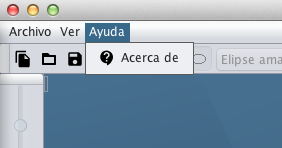
\includegraphics[width=0.3\textwidth]{generales/ayuda2.png}
  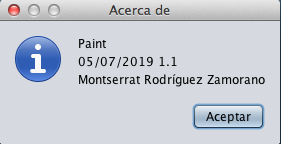
\includegraphics[width=0.3\textwidth]{generales/ayuda1.png}
 \caption{Diálogo con el nombre del programa, versión y autor}
 \label{diseño}
 \end{figure}
\subsection{Gráficos}
\subsection{Barra de atributos}
La barra de atributos servirá para seleccionar las características para pintar la próxima figura y para modificarlas. Sin embargo, facilitará su uso al usuario inhabilitando aquellos elementos que no pueden utilizarse con las opciones seleccionadas.
\vskip0.3cm
Por ejemplo, no tiene sentido que las opciones de relleno estén activadas cuando estamos dibujando una línea.
\begin{figure}[H]
 \centering
  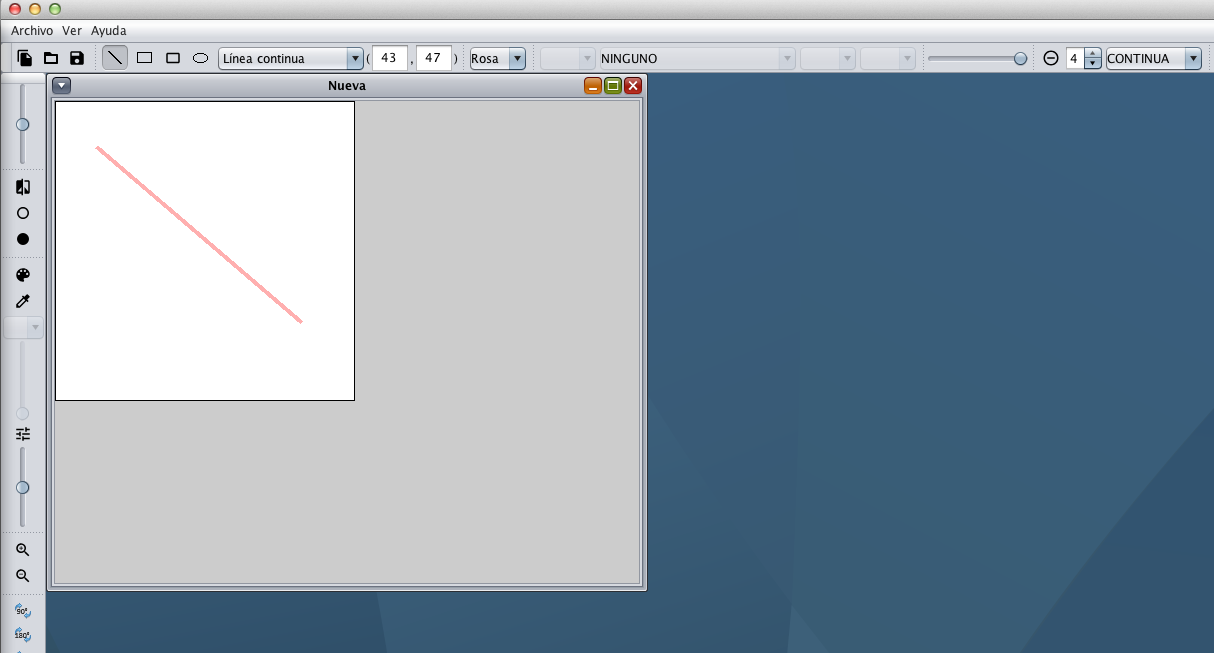
\includegraphics[width=0.8\textwidth]{graficos/coherencia1.jpg}
 \caption{Los elementos se activan/desactivan en función de las características de la figura que seleccionamos}
 \label{diseño}
 \end{figure}
 También se lanzarán mensajes de error si intentamos dibujar una figura sin haber seleccionado todos sus argumentos: por ejemplo, si indicamos que la figura está rellena pero no seleccionamos un color de relleno.
 \begin{figure}[H]
 \centering
  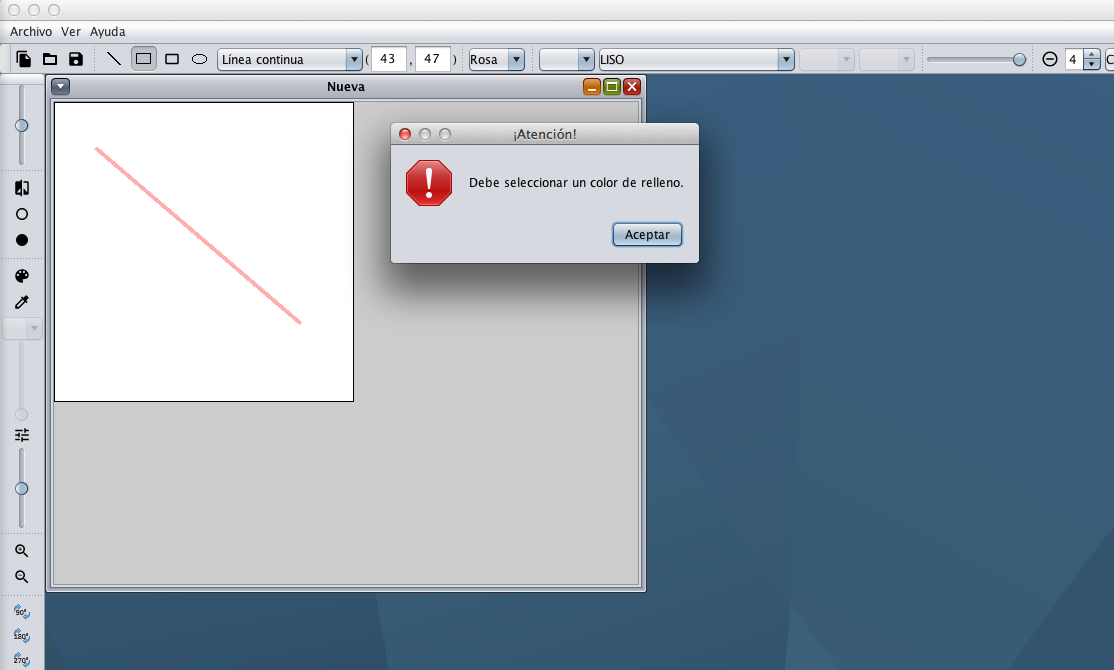
\includegraphics[width=0.8\textwidth]{graficos/coherencia2.jpg}
 \caption{Mensajes de advertencia en el dibujado de las figuras}
 \label{diseño}
 \end{figure}
En este aspecto hay un problema: se ha tenido ciertos problemas con las listas desplegables. En particular, no hay una opción de no línea o línea nula, por lo que aunque al crear o abrir una imagen aparezca seleccionada la opción de línea continua, es necesario seleccionarla para que realmente se inicialice el objeto.\vskip0.3cm
 Algo parecido pasa con los colores: si se abre el ComboBox, aunque no se seleccione ningún color, si se vuelve a cerrar se seleccionará el color negro. Es necesario hacer clic sobre uno de los colores para que se pueda crear la figura.
\subsubsection{Selección de una figura}
Comprobamos que cuando se selecciona una figura, sus atributos se seleccionan automáticamente y correctamente en la barra de herramientas. Para seleccionar una figura, hay que seleccionar la ventana que contiene la imagen en la que está la figura deseada y buscarla en la lista desplegable de figuras.
\vskip0.3cm
\begin{figure}[H]
 \centering
  \includegraphics[width=0.8\textwidth]{graficos/seleccionFigura.jpg}
 \caption{Selección de una figura}
 \label{diseño}
 \end{figure}
 \subsubsection{Editar los atributos de una figura}
 Se comprueba que pueden modificarse las propiedades de una figura. Para hacerlo, solo hay que seleccionar la figura a modificar y seleccionar los atributos deseados.
 \vskip0.3cm
\begin{figure}[H]
 \centering
  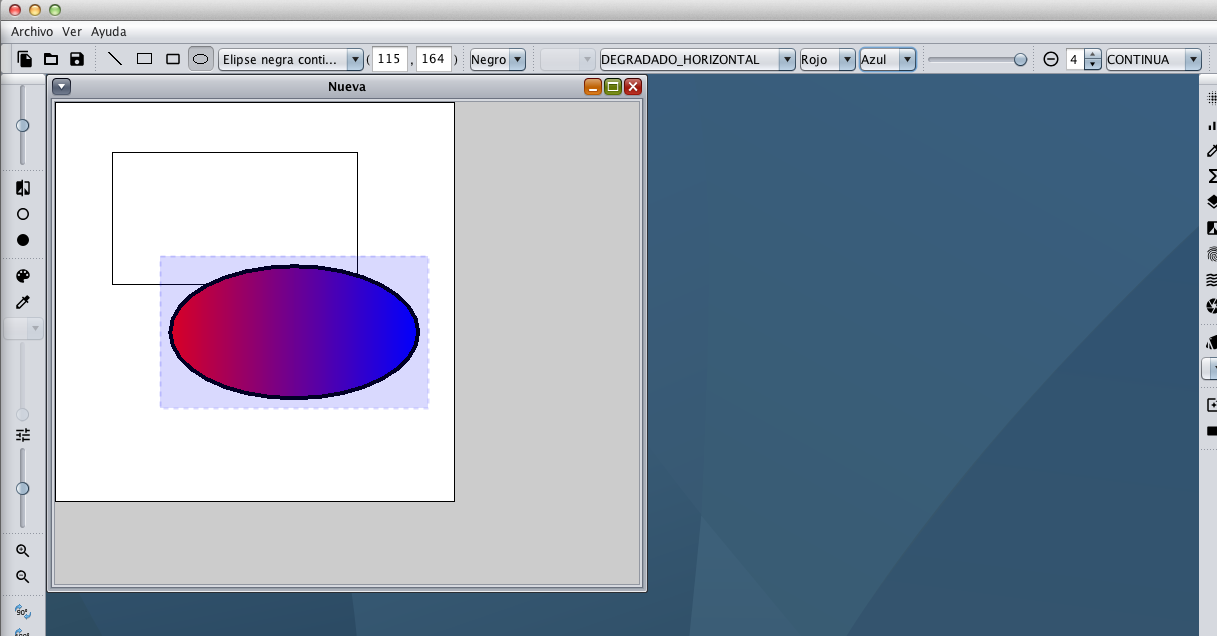
\includegraphics[width=0.4\textwidth]{graficos/cambioAtributos1.png}
  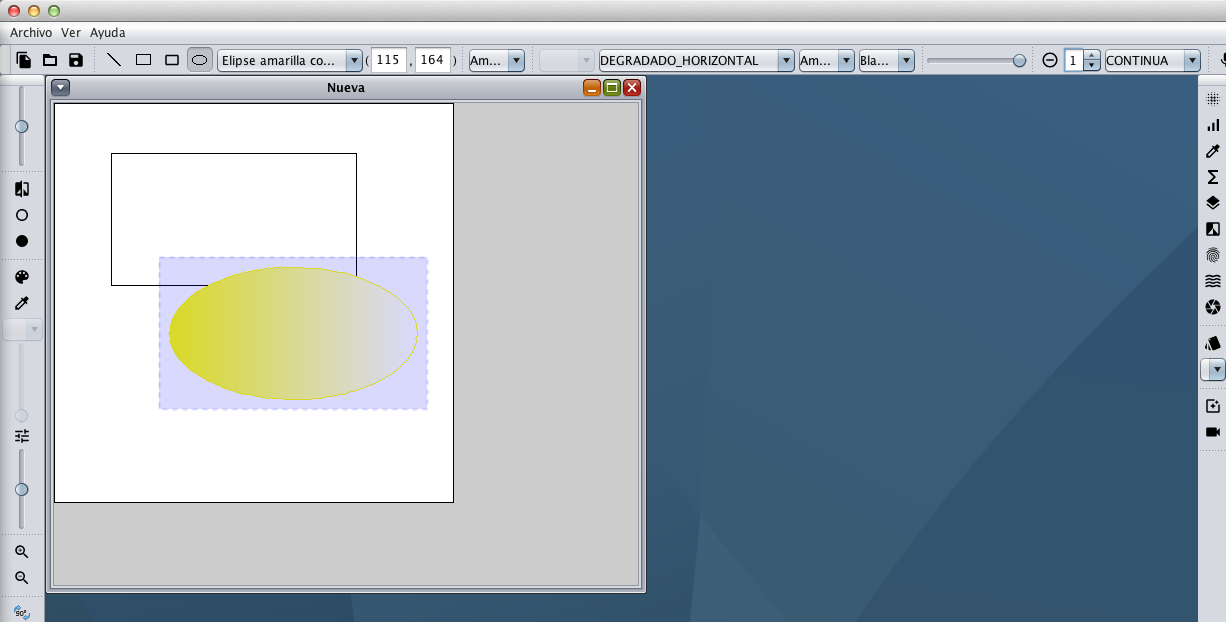
\includegraphics[width=0.4\textwidth]{graficos/cambioAtributos2.png}
 \caption{Cambio de atributos de una imagen}
 \label{diseño}
 \end{figure}
\vskip0.3cm
La posición es un atributo más de la figura. Como se puede ver, se puede seleccionar la figura y moverla. Para ello hay que introducir la posición en los campos de texto habilitados para ello (señalados en la imagen con el círculo amarillo).
 \vskip0.3cm
\begin{figure}[H]
 \centering
  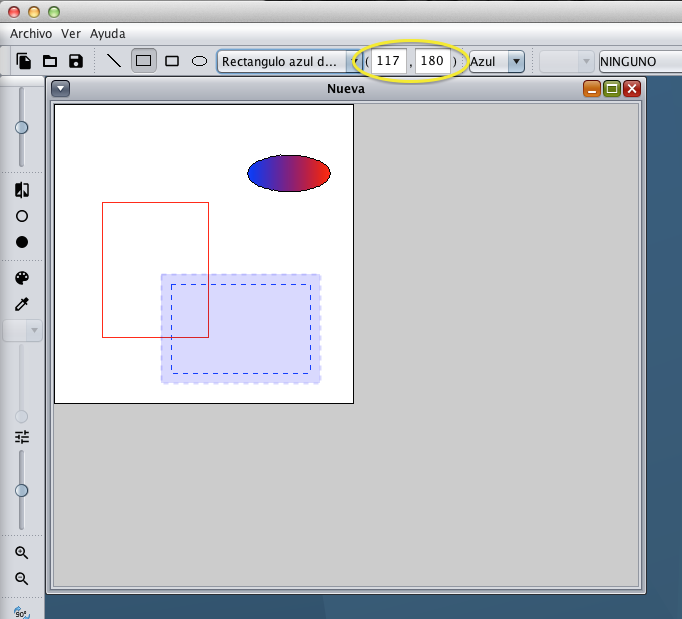
\includegraphics[width=0.4\textwidth]{graficos/mover1.png}
  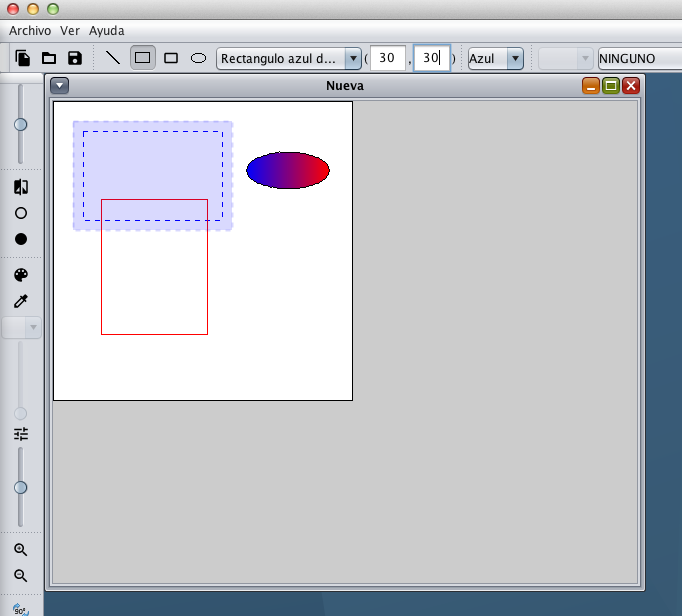
\includegraphics[width=0.4\textwidth]{graficos/mover2.jpg}
 \caption{Mover figura}
 \label{diseño}
 \end{figure}
\subsection{Procesamiento de imágenes}
A continuación se probarán los diferentes filtros disponibles en la aplicación.
\subsubsection{Duplicar}
Se comprobará si la duplicación de la imagen se ha realizado correctamente, de forma que si se modifica una, los cambios no se aplican en la otra.
\vskip0.3cm
\begin{figure}[H]
 \centering
  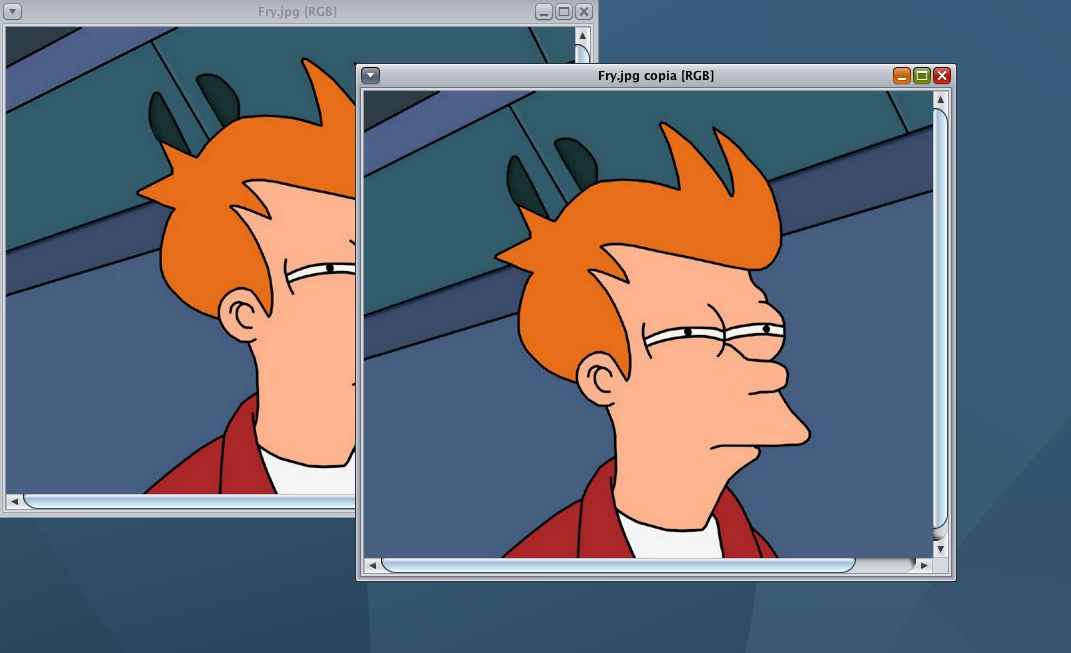
\includegraphics[width=0.5\textwidth]{imagenes/duplicar1.png}
  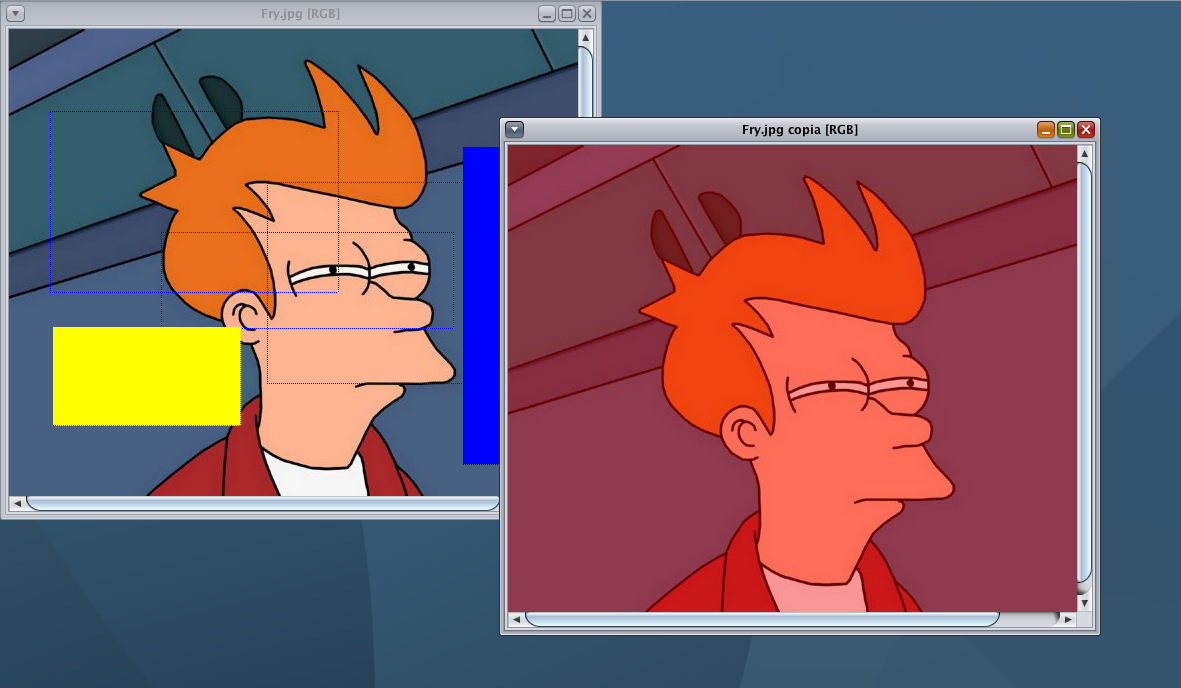
\includegraphics[width=0.5\textwidth]{imagenes/duplicar2.jpg}
 \caption{Duplicar imagen}
 \label{diseño}
 \end{figure}
\subsubsection{Modificar brillo}
\vskip0.3cm
\begin{figure}[H]
 \centering
  
\includegraphics[width=0.3\textwidth]{imagenes/fryBrilo2.jpg}
  \includegraphics[width=0.3\textwidth]{imagenes/Fry.jpg}
  \includegraphics[width=0.3\textwidth]{imagenes/fryBrillo1.jpg}
 \caption{Modificación del brillo}
 \label{diseño}
\end{figure}
\subsubsection{Filtro de emborronamiento}
Se ha aplicado varias veces el filtro para que sea visible.
\vskip0.3cm
\begin{figure}[H]
 \centering
  \includegraphics[width=0.3\textwidth]{imagenes/Fry.jpg}
  \includegraphics[width=0.3\textwidth]{imagenes/fryEmborronamiento.jpg}
 \caption{Aplicación filtro emborronamiento}
 \label{diseño}
\end{figure}
\subsubsection{Filtro de enfoque}
\vskip0.3cm
\begin{figure}[H]
 \centering
  \includegraphics[width=0.3\textwidth]{imagenes/Fry.jpg}
  \includegraphics[width=0.3\textwidth]{imagenes/fryEnfoque.jpg}
 \caption{Aplicación filtro enfoque}
 \label{diseño}
\end{figure}
\subsubsection{Filtro de relieve}
\vskip0.3cm
\begin{figure}[H]
 \centering
  \includegraphics[width=0.3\textwidth]{imagenes/Fry.jpg}
  \includegraphics[width=0.3\textwidth]{imagenes/fryRelieve.jpg}
 \caption{Aplicación filtro relieve}
 \label{diseño}
\end{figure}
\subsubsection{Contraste normal}
\vskip0.3cm
\begin{figure}[H]
 \centering
  \includegraphics[width=0.3\textwidth]{imagenes/Fry.jpg}
  \includegraphics[width=0.3\textwidth]{imagenes/fryContraste.jpg}
 \caption{Aplicación contraste}
 \label{diseño}
\end{figure}
\subsubsection{Iluminado}
\vskip0.3cm
\begin{figure}[H]
 \centering
  \includegraphics[width=0.3\textwidth]{imagenes/Fry.jpg}
  \includegraphics[width=0.3\textwidth]{imagenes/fryIluminado.jpg}
 \caption{Aplicación iluminación}
 \label{diseño}
\end{figure}
\subsubsection{Oscurecido}
\vskip0.3cm
\begin{figure}[H]
 \centering
  \includegraphics[width=0.3\textwidth]{imagenes/Fry.jpg}
  \includegraphics[width=0.3\textwidth]{imagenes/fryOscurecido.jpg}
 \caption{Aplicación oscurecido}
 \label{diseño}
\end{figure}
\subsubsection{Invertir colores}
\vskip0.3cm
\begin{figure}[H]
 \centering
  \includegraphics[width=0.3\textwidth]{imagenes/Fry.jpg}
  \includegraphics[width=0.3\textwidth]{imagenes/fryNegativo.jpg}
 \caption{Aplicación filtro negativo}
 \label{diseño}
\end{figure}
\subsubsection{Conversión a espacios RGB, YCC, GRAY}
Para comprobar que la conversión se ha realizado correctamente, se extraen las bandas de colores y se comparan. En la imagen se pueden ver la tercera banda de una imagen en espacio de color RGB y YCC, respectivamente.
\vskip0.3cm
\begin{figure}[H]
 \centering
  \includegraphics[width=0.3\textwidth]{imagenes/banda3RGB.jpg}
  \includegraphics[width=0.3\textwidth]{imagenes/banda3YCC.jpg}
 \caption{}
 \label{diseño}
\end{figure}
\subsubsection{Giro libre}
\vskip0.3cm
\begin{figure}[H]
 \centering
  \includegraphics[width=0.3\textwidth]{imagenes/Fry.jpg}
  \includegraphics[width=0.3\textwidth]{imagenes/fryGiro.jpg}
 \caption{Giro libre}
 \label{diseño}
\end{figure}
\subsubsection{Escalado}
\vskip0.3cm
\begin{figure}[H]
 \centering
  \includegraphics[width=0.5\textwidth]{imagenes/escalado.png}
 \caption{Escalado de la imagen}
 \label{diseño}
\end{figure}
\subsubsection{Tintado}
\vskip0.3cm
\begin{figure}[H]
 \centering
  \includegraphics[width=0.3\textwidth]{imagenes/fryTinteRojo.jpg}
  \includegraphics[width=0.3\textwidth]{imagenes/Fry.jpg}
  \includegraphics[width=0.3\textwidth]{imagenes/fryTinteAmarillo.jpg}
 \caption{Tintado de la imagen}
 \label{diseño}
\end{figure}
\subsubsection{Ecualización}
\vskip0.3cm
\begin{figure}[H]
 \centering
  \includegraphics[width=0.3\textwidth]{imagenes/Fry.jpg}
  \includegraphics[width=0.3\textwidth]{imagenes/fryEcualizacion.jpg}
 \caption{Aplicación ecualización}
 \label{diseño}
\end{figure}
\subsubsection{Filtro sepia}
\vskip0.3cm
\begin{figure}[H]
 \centering
  \includegraphics[width=0.3\textwidth]{imagenes/Fry.jpg}
  \includegraphics[width=0.3\textwidth]{imagenes/frySepia.jpg}
 \caption{Aplicación filtro sepia}
 \label{diseño}
\end{figure}
\subsubsection{Umbralización}
\vskip0.3cm
\begin{figure}[H]
 \centering
  \includegraphics[width=0.3\textwidth]{imagenes/Fry.jpg}
  \includegraphics[width=0.3\textwidth]{imagenes/fryUmbralizado.jpg}
 \caption{Umbralizar imagen}
 \label{diseño}
\end{figure}
\subsubsection{Operador \textit{LookupOp} basado en una función propia}
\begin{figure}[H]
 \centering
  \includegraphics[width=0.3\textwidth]{imagenes/Fry.jpg}
  \includegraphics[width=0.3\textwidth]{imagenes/fryCos.jpg}
 \caption{Operación cosinusoide}
 \label{diseño}
 \end{figure}
\subsubsection{Operación de diseño propio: filtro violeta}
\vskip0.3cm
\begin{figure}[H]
 \centering
  \includegraphics[width=0.3\textwidth]{imagenes/Fry.jpg}
  \includegraphics[width=0.3\textwidth]{imagenes/fryVioleta.jpg}
 \caption{Aplicación filtro violeta}
 \label{diseño}
 \end{figure}
\subsection{Sonido}
\subsubsection{Reproducción de sonido}
A continuación se muestran las funcionalidades del sonido. Como se puede comprobar, cuando se activa el sonido, no estarán activos los botones para el procesamiento de imágenes.
\vskip0.3cm
\begin{figure}[H]
 \centering
  \includegraphics[width=0.5\textwidth]{sonido/archivoAbierto.png}
 \caption{Abrir archivo de sonido}
 \label{diseño}
 \end{figure}
Como puede verse, si el archivo de audio no está reproduciéndose no podrán pulsarse el botón de parada. El botón de pausa no estará disponible para el sonido.
\subsubsection{Grabación de sonido}
El programa nos permitirá también grabar sonido. Una vez que se comience la grabación se deshabilitará el botón de grabar y se activará el de detener a grabación.
\vskip0.3cm
\begin{figure}[H]
 \centering
  \includegraphics[width=0.5\textwidth]{sonido/grabacion1.png}
  \includegraphics[width=0.5\textwidth]{sonido/grabacion2.png}
 \caption{Grabar/Detener grabación}
 \label{diseño}
 \end{figure}
 Una vez que se haya detenido la grabación, se podrá guardar. Será necesario escribir la extensión cuando se guarde el archivo (\texttt{au} o \texttt{wav}). Un vez guardada la grabación, se añadirá a la lista de audios y se podrá reproducir.
 \vskip0.3cm
\begin{figure}[H]
 \centering
  \includegraphics[width=0.5\textwidth]{sonido/grabacion3.png}
  \includegraphics[width=0.5\textwidth]{sonido/grabacion4.png}
 \caption{Guardar grabación}
 \label{diseño}
 \end{figure}
\subsection{Vídeo}
A continuación se muestran las funcionalidades del vídeo y la cámara. Como se puede comprobar, cuando se activa la WebCam, no estarán activos los botones para el procesamiento de imágenes.
\subsubsection{WebCam}
En primer lugar, comprobamos que puede abrirse correctamente la cámara. Una vez hecho esto, se comprobará si se realizan las capturas de pantalla correctamente. Si no hay ventana de cámara abierta, no se podrá sacar ninguna captura de pantalla.
\vskip0.3cm
\begin{figure}[H]
 \centering
  \includegraphics[width=0.8\textwidth]{video/webcam.jpg}
 \caption{Webcam abierta}
 \label{diseño}
 \end{figure}
 \vskip0.3cm
\begin{figure}[H]
 \centering
  \includegraphics[width=0.8\textwidth]{video/captura.jpg}
 \caption{Captura de pantalla}
 \label{diseño}
 \end{figure}
 
\section{Mejoras para posteriores versiones}
\begin{itemize}
\item{El botón de reproducir no se desactiva aunque esté programado en los manejadores de audio y de vídeo.}
\item{Mejorar las listas desplegables de relleno y tipo de línea añadiendo dibujos o iconos.}
\item{Buscar una alternativa para el vídeo disponible para todos los sitemas operativos.}
\end{itemize}

%\begin{lstlisting}[language=python, caption=Código gradiente descendente, label=lst:graddesc]
%\end{lstlisting}
%\renewcommand{\labelenumi}{\alph{enumi})}

%%BIBLIOGRAFIA%%
\clearpage
\begin{thebibliography}{X}
\bibitem{} Apuntes de la asignatura y guiones de prácticas.\\
\url{https://decsai.ugr.es}
\bibitem{} Documentación Java \\ \url{https://docs.oracle.com/javase/7/docs/api/java/awt/}
\bibitem{} Tutoriales para el uso de vlcj \\ \url{http://capricasoftware.co.uk/projects/vlcj-4/tutorials}
\bibitem{} Código para ComboBoxs personalizados 
\url{https://docs.oracle.com/javase/8/docs/api/javax/swing/ListCellRenderer.html}
\end{thebibliography}
\end{document}
